\documentclass[11pt, a4paper, oneside]{Packages/Thesis}
\graphicspath{{Pictures/}}
\usepackage[square, numbers, comma, sort&compress]{natbib}
\hypersetup{urlcolor=black, colorlinks=true}
\setlength{\parindent}{1cm}
\title{\ttitle}
\begin{document}
\frontmatter % Use roman page numbering style (i, ii, iii, iv...) for the pre-content pages
\setstretch{1.3} % Line spacing of 1.3

\fancyhead{} % Clears all page headers and footers
\rhead{\thepage} % Sets the right side header to show the page number
\lhead{} % Clears the left side page header

\pagestyle{fancy} % Finally, use the "fancy" page style to implement the FancyHdr headers
%
\newcommand{\HRule}{\rule{\linewidth}{0.5mm}} % New command to make the lines in the title page

% PDF meta-data
\hypersetup{pdftitle={\ttitle}}
\hypersetup{pdfsubject=\subjectname}
\hypersetup{pdfauthor=\authornames}
\hypersetup{pdfkeywords=\keywordnames}

%----------------------------------------------------------------------------------------
%	TITLE PAGE
%----------------------------------------------------------------------------------------

\begin{titlepage}
\begin{center}

\textsc{\LARGE \univname}\\[0.1cm] % University name
\textsc{\large \facname\\\deptname}\\[1cm] % Research group name and department name

\begin{minipage}{\linewidth}
	\centering
	\begin{minipage}{0.45\linewidth}
		\begin{figure}[H]
			
\includegraphics[width=.4\linewidth, left]{Pictures/UCL/ucl.jpg}
		\end{figure}
	\end{minipage}
	\hspace{0.05\linewidth}
	\begin{minipage}{0.45\linewidth}
		\begin{figure}[H]
			
\includegraphics[width=.5\linewidth, right]{Pictures/UCL/epl.jpg}
		\end{figure}
	\end{minipage}
\end{minipage}\\[1cm]

\textsc{\Large Master thesis}\\[1cm] % Thesis type

\HRule \\[0.4cm] % Horizontal line
{\huge \bfseries \ttitle}\\[0.4cm] % Thesis title
\HRule \\[1.5cm] % Horizontal line
 
\begin{minipage}{0.4\textwidth}
\begin{center} \large
\emph{Authors:}\\
{\authornames} % Author name - remove the \href bracket to remove the link
\end{center}
\end{minipage}
\\[3cm]
\noindent{\large \emph{Thesis Supervisor} \hfill Thesis submitted to obtain}\\
\noindent{\large {\supname} \hfill the degree of \textit{\degreename} in}\\
\noindent{\large \emph{Readers} \hfill \textit{computer science} with option}\\
\noindent{\large Quentin \textsc{Hunin} \hfill in \textit{networking and security}}\\
\noindent{\large David \textsc{Lebrun} \hfill \vspace{10mm}}\\[1.5cm] % University requirement text
 
{\large Louvain-la-Neuve\\ June 2014}\\[4cm] % Date
%\includegraphics{Logo} % University/department logo - uncomment to place it
 
\vfill
\end{center}

\end{titlepage}

\clearpage
%----------------------------------------------------------------------------------------
%	QUOTATION PAGE
%----------------------------------------------------------------------------------------
\pagestyle{empty} % No headers or footers for the following pages

\null\vfill % Add some space to move the quote down the page a bit

We would like to specially thanks Olivier Bonaventure, Dominique Margot and Quentin Hunin from the UCL SRI team  for their availability, support and help during the realization of this project.

%\begin{flushright}
%Dave Barry
%\end{flushright}

\vfill\vfill\vfill\vfill\vfill\vfill\null % Add some space at the bottom to position the quote just right

\clearpage % Start a new page

%----------------------------------------------------------------------------------------
%	LIST OF CONTENTS/FIGURES/TABLES PAGES
%----------------------------------------------------------------------------------------

\pagestyle{fancy} % The page style headers have been "empty" all this time, now use the "fancy" headers as defined before to bring them back

\lhead{\emph{Contents}} % Set the left side page header to "Contents"
\tableofcontents % Write out the Table of Contents


%----------------------------------------------------------------------------------------
%	THESIS CONTENT - CHAPTERS
%----------------------------------------------------------------------------------------

\mainmatter % Begin numeric (1,2,3...) page numbering

\pagestyle{fancy} % Return the page headers back to the "fancy" style
\nocite{*}
% Include the chapters of the thesis as separate files from the Chapters folder
% Uncomment the lines as you write the chapters
% Chapter Template

\chapter{Introduction} % Main chapter title

\label{Chapter1} % Change X to a consecutive number; for referencing this chapter elsewhere, use \ref{ChapterX}

\lhead{Chapter 1. \emph{Introduction}} % Change X to a consecutive number; this is for the header on each page - perhaps a shortened title

%\section{Presentation}
%This project constitute our master thesis. The goal is to implement a set of tools to help the network administrators monitoring the wireless infrastructure. To achieve that, we have to proceed in two steps. First, we will have to collect all the information available. The sources of information are completely heterogeneous. They range from simple logs to active monitoring through customized routers. The main difficulty here will be to aggregate all the information in a coherent and efficient way. The amount of data will force us to choose which ones are pertinent and which ones are not. Once the gathering steps is done, the raw data will be available but they will be useless if the user can't understand and use them. So, the second step will be to analyse and present them to the users. We will have to define the profile of the end-user and understand what are his needs. The success of our work will be directly link to the fact if our implementation is helpful or not. If the data collected are correct but we are unable to present them in the right way, our work would be meaningless.


\section{Towards a WiFi Monitoring Tool}
As for other universities around the world, the Catholic Univeristy of Louvain has a large wireless network throughout its different campus. This network provides a direct and reliable connection to all the students, staff, teachers and researchers of the university at all time. The problem with the UCL infrastructure is that it is quite huge and it is always changing. The UCL/SRI team, which is responsible for the effective development of that infrastructure and its connection with the outside world, is always trying to improve the connectivity on the site by adding access point or upgrading the Cisco controllers.\\

Because of that complexity, the management and the efficiency of that network has become quite difficult and buggy. Indeed, the logfiles produced by the controllers are very verbose which induce an arduous and tricky work of decryption when a the team wants to find and trace a problem that occured before on the system. Furthermore, there are more and more users trying to get a connection on the campus (laptops, smartphones,...). This might causes some disturbance on the network that leads to connectivity problems for the direct user.\\

In this thesis, we discuss the implementation of a WiFi monitoring tool that will help the network administrators managing the wireless infrastructure. To achieve that, we have to proceed in two steps. First of all, we have to collect all the information that travels over the network. Those information come from heterogeneous sources (from controllers logfiles to active monitoring logs through customized routers). Second, we have to analyze and process that raw data in a way that is understandable and readable for the end users.

\subsection{Data Gathering}
As said before, the sources of data are quite heterogeneous. To handle that, we'll have to implement a system that can hold and represent all the information in a consistent way.

\subsection{Data Analysis}
The core will be responsible to centralized, analyse and take the action accordingly the information received from the probes. Its actions will mainly depend on the access that it will have the network. Typical action would be to adapt the controller or inform precisely the administrator of the problems detected. Most of the time, there most difficult is not to be aware of the problem but to understand the causes of it.

Throughout this thesis we explain what are the main issues encountered today on the university wireless network and how our monitoring tool is helping the network administrators managing this system. In a first chapter, we present the working environment, and more specifically, the UCL Internet infrastructure. We also discuss the different types of logs we use in our tool. In the following chapter, we present all the network components and protocols used inside the network and where connectivity problems can occur. Finally we provide and describe an implementation of our monitoring tool and we deploy it on the network to gather results and feedback.





\section{Motivation}

\section{Objectives}
% Chapter Template

\chapter{Working Environment} % Main chapter title

\label{Chapter2} % Change X to a consecutive number; for referencing this chapter elsewhere, use \ref{ChapterX}

\lhead{Chapter 2. \emph{Working Environment}} % Change X to a consecutive number; this is for the header on each page - perhaps a shortened title

%----------------------------------------------------------------------------------------
%	SECTION 1
%----------------------------------------------------------------------------------------

%http://www.cisco.com/web/FR/documents/pdfs/livres_blancs/mobilite_sans_fil/Protocole_LWAPP.pdf

\section{UCL's Wireless Infrastructure}

On its Louvain-la-Neuve's campus area, the Catholic University of Louvain offers five different networks, each with a different \texttt{SSID}, that are reserved to certain parts of users according to their category. These available networks are the following:
\begin{itemize}
	\item[-] \texttt{student.UCLouvain}: Available for all the students enrolled at the Catholic University of Louvain.
	\item[-] \texttt{UCLouvain}: Reserved for the university's staff
	\item[-] \texttt{UCLouvain-prive}: Limited access to check the UCL's wireless configuration page or to download required programs for Windows XP and Windows Vista.
	\item[-] \texttt{visiteurs.UCLouvain}: Accessible for guests invited by the university.
	\item[-] \texttt{eduroam}: International education roaming access.
\end{itemize}

Network security is an important issue and an everyday struggle at the university and several measures are regularly taken by the SGSI team in order to keep the integrity and the consistency of the UCL's network preserved. As an example, Microsoft has decided on the 8th of April 2014 to end the Windows XP's support and updates leaving all the remaining laptops running this operating system unprotected to possible external threats \cite{windows}. The problem with that Microsoft's decision is that those outdated computers might become more vulnerable to security risks and malwares/viruses. It could turn into a real problem for the university's network because if a contaminated host is able to connect to the network it can cause serious damages to the overall infrastructure. In order to counter this possible problem, the SGSI team plan to block the wireless access using, for example, snorting programs, to any device that still runs on Windows XP.

The main way of protecting the UCL's network infrastructure from exterior threats that has been installed and configured by the SGSI team is the use of the \texttt{IEEE 802.1X} standard providing an authentication mechanism for all the devices that want to connect to one of the UCL's wireless networks. This architecture uses an authentication with user ID and password. Basically, every student, professor, researcher or staff members needs a \textit{username} and a \textit{password} in order to be able to establish a connection with one of the networks and get access to the Internet inside the UCL's campus. The username is composed of two parts, on one side the login the user has received from the university's administrative system when he enrolled himself, and on the other side the realm (\texttt{@wifi.uclouvain.be}). Along with that username, the user also needs a password. This password is the same as the password he uses to connect to his personal virtual office on the university's web site. Without those credentials it is impossible for him get an Internet connection within the university's campus.

This kind of authentication mechanism is only possible if the infrastructure has several key entities that are going to handle all this security authentication process. Those entities are an \textit{Authentication Server} and an \textit{Authenticator}.

Typically an Authentication Server is a host that supports the \texttt{RADIUS} and  \texttt{EAP} protocols. In the case of the UCL's infrastructure the Authenticator Server is also composed of several database servers, placed behind a load balancer, that support the \texttt{LDAP}\footnote{Lightweight Directory Access Protocol} protocol and where all the information about the students, professors, researchers and staff members of the UCL as well as a lot of other data are stored. Among those stored data, we find all the users' credentials.

The Authenticator is composed of the access point that handles the connection request from the user and the Cisco controller that handles all the authentication process. This authenticator is the real security guard for the network since the client is not allowed to access to the protected side of the network until it's identity has been checked and validated. Let's keep in mind that these controller and access point do not play a role in the real world of the authentication itself. They are called the \textit{Authenticator} because that is where the client asks for authentication but they do not authenticate the client. The device that authenticate the client is the \textit{Authentication Server}.

The following figure represents the architecture with the different components that handles the \texttt{802.1X} authentication process at the UCL. 

\begin{figure}[H]
	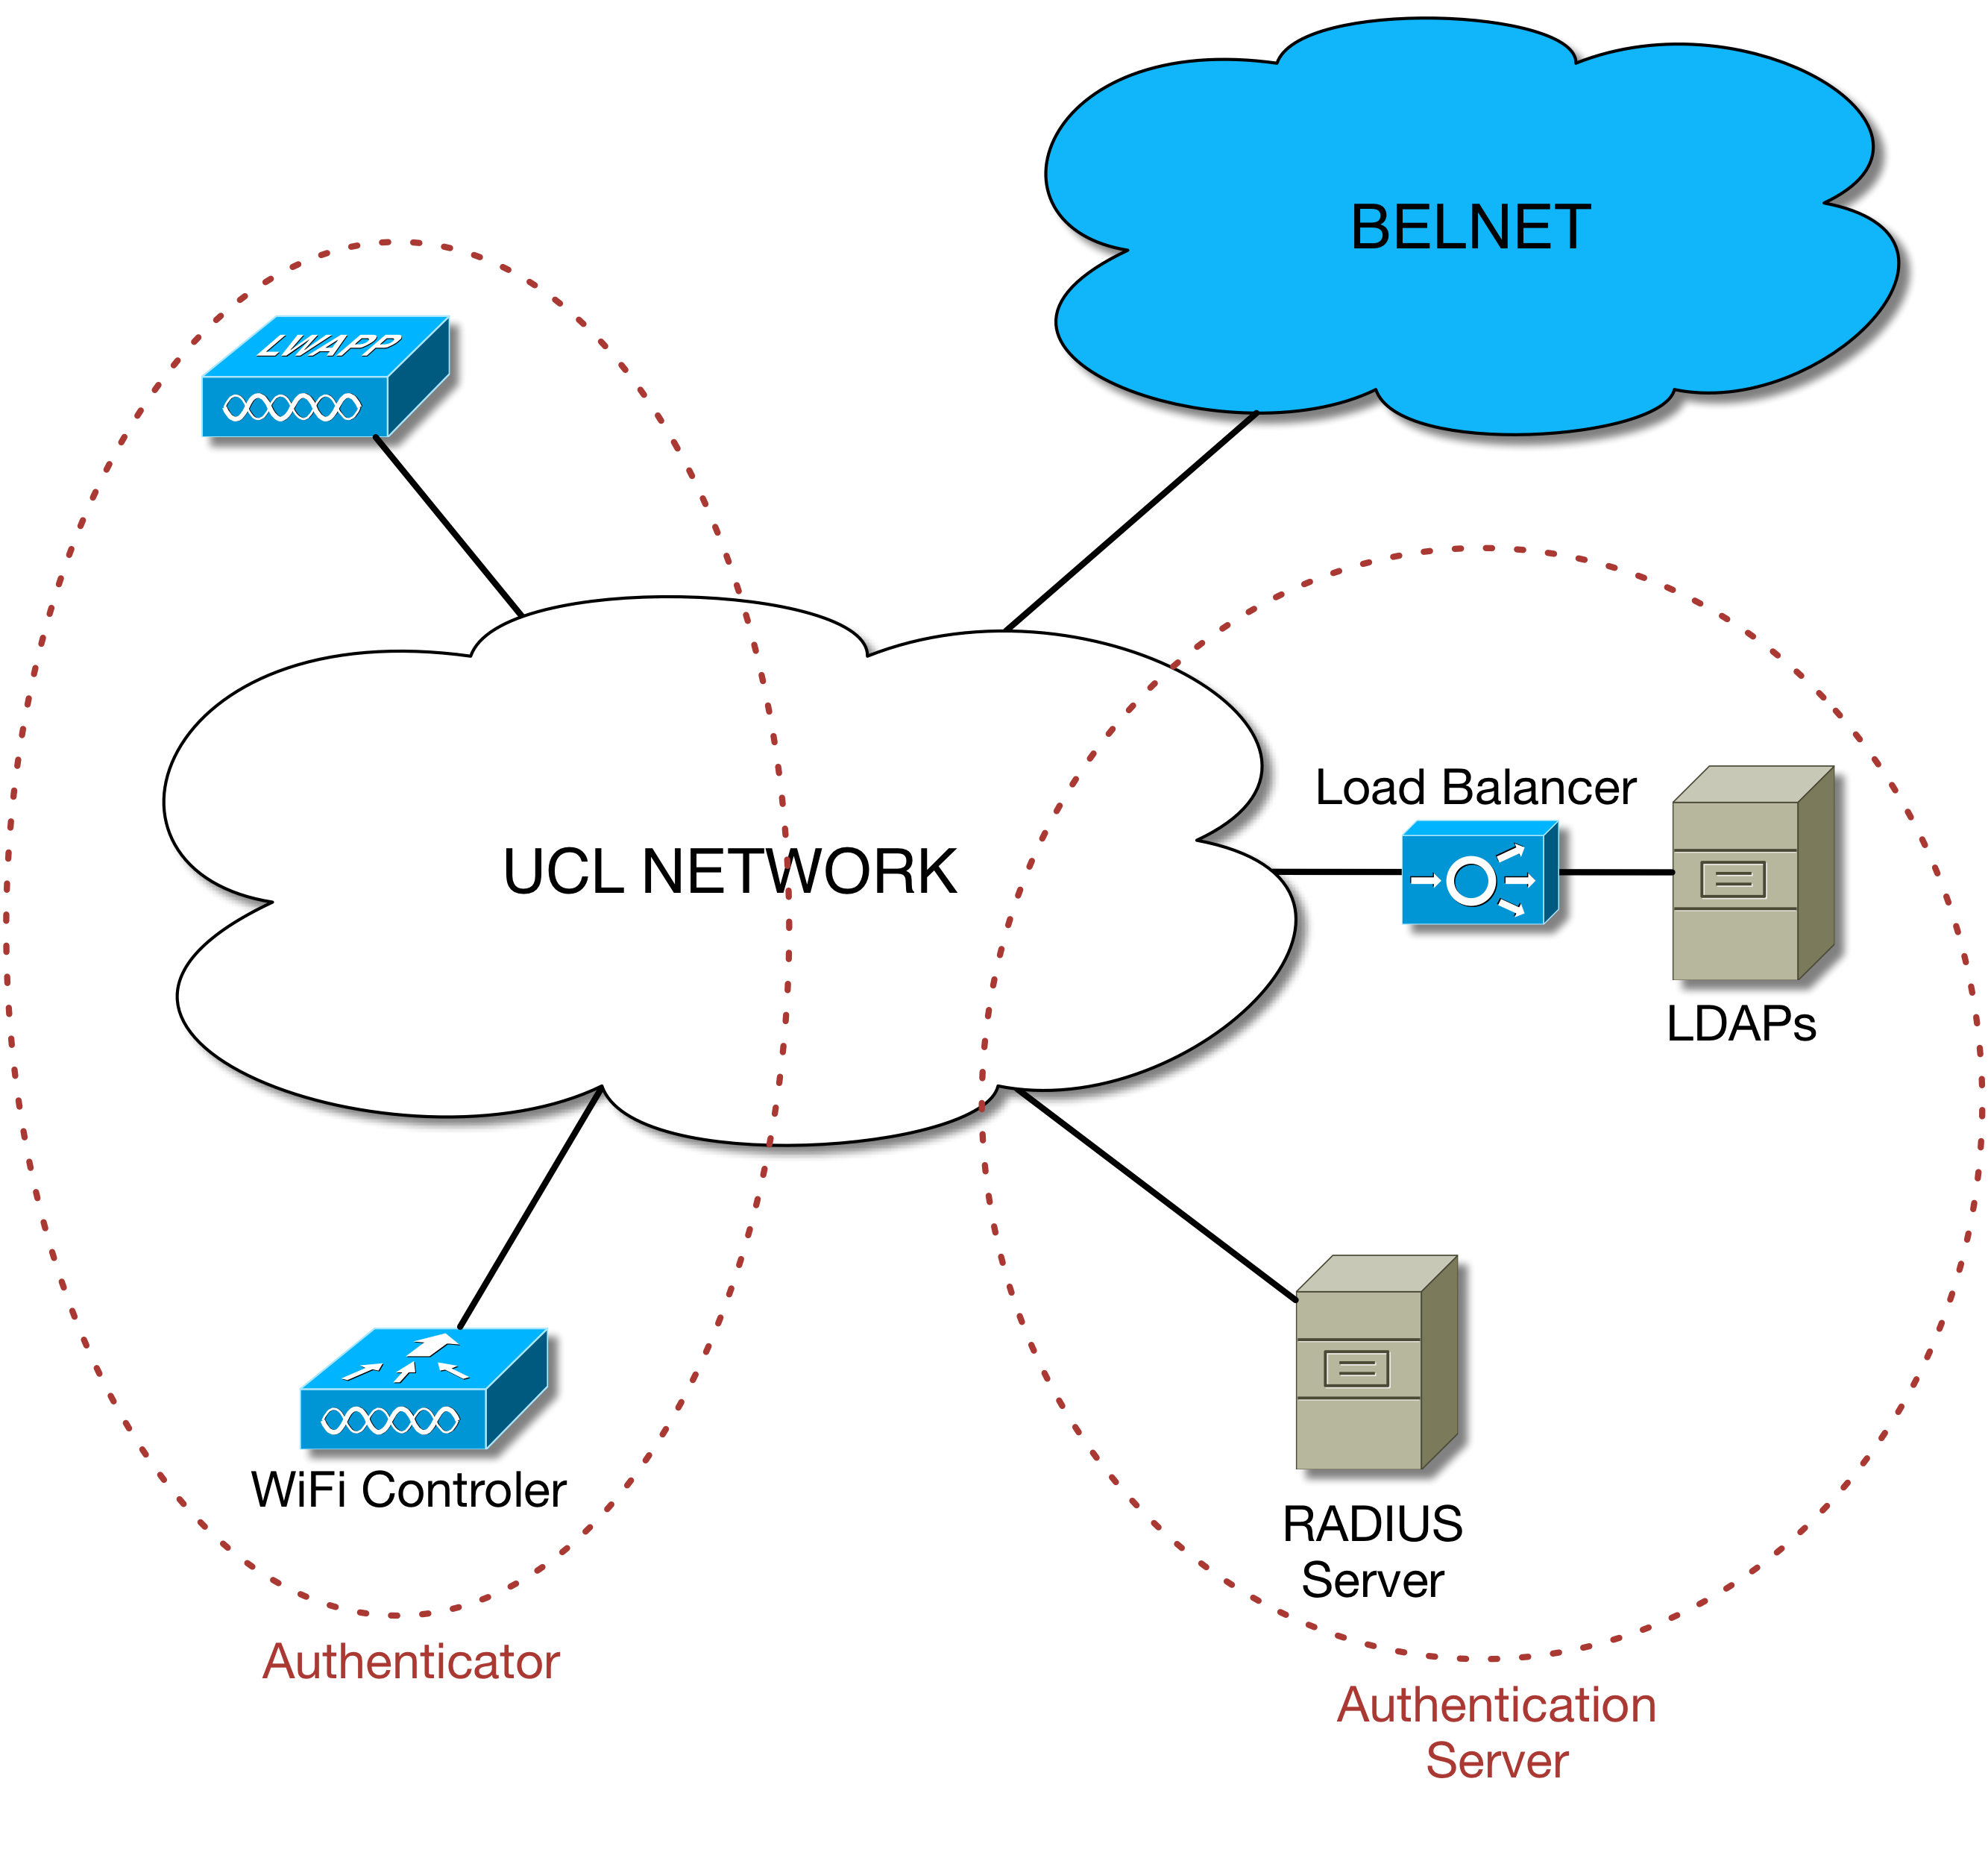
\includegraphics[width=1\linewidth]{Pictures/chapter2/802-archi.png}
	\caption{\texttt{802.1X} architecture and components at the UCL}
\end{figure}



\section{Network Components and Protocols}
In this section, we give more information and details about all the protocols and components used throughout this thesis.

\subsection{EAP}
The Extensible Authentication Protocol is an Internet Engineering Task Force (IETF) flexible authentication framework standard defined in the \texttt{RFC3748} \cite{rfc3748}. \texttt{EAP} was designed to work without the IP protocol and provides support only for the transport of authentication protocols. This protocol runs directly over data link layers such as \texttt{Point-to-Point Protocol} (PPP) or \texttt{IEEE 802}. It is used to select a specific authentication mechanism whenever the authenticator requests more information to the supplicant.

The particularity with \texttt{EAP} is that the authentication mechanism is negotiated by the peers (i.e. the supplicants) during the connection authentication phase with the authentication server. The peers negotiate the use of which \texttt{EAP} method to use during the authentication. Once the method has been agreed upon, an \texttt{EAP} conversation consisting of requests and responses messages exchanged between the peer and the authentication server starts.

The \texttt{EAP} architecture consists of three main elements:
\begin{itemize}
	\item \textbf{EAP peer}: The peer is the client that tries to access the protected network and that responds to the authenticator requests.
	\item \textbf{EAP authenticator}: It is the end of the link initiating an \texttt{EAP} authentication process. It is the access point or the network access server that requires \texttt{EAP} authentication in order to grant access to the network.
	\item \textbf{Authentication server}: The server that communicates with the \texttt{EAP} peer. It negotiate the \texttt{EAP} method to use and validates the peer's credentials allowing it to access the protected network or not.
\end{itemize}

Since \texttt{EAP} only defines message formats it has to be encapsulated inside a data link layer transport protocols. Between the peer and the authenticator, the \texttt{EAP} messages has to be encapsulated inside protocols such as \texttt{PPP}, \texttt{PEAP} or \texttt{IEEE 802.1X}. The encapsulation of \texttt{EAP} over \texttt{IEEE 802.1X} is called \texttt{EAPOL}\footnote{EAP over LANs}. Once the authenticator has received a \texttt{EAP} message from the peer, it has to forward it to the authentication server and it does that by encapsulating the message using that \texttt{RADIUS} protocol. Thanks to that, the \texttt{EAP} messages are exchanged between the peer and the authentication server smoothly. Since the information flows between those two entities, the authenticator does not need to support any of the \texttt{EAP} methods. It just has to forward the messages.

The following figure\footnote{http://technet.microsoft.com/en-us/library/bb457039.aspx} shows the \texttt{EAP} infrastructure and the information flow between the three components.

\begin{figure}[H]
	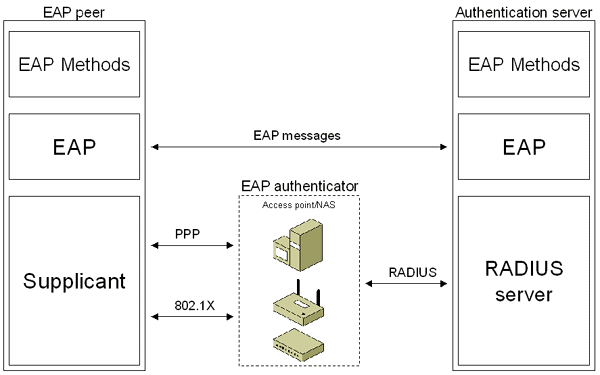
\includegraphics[width=1\linewidth]{Pictures/chapter2/eap.png}
	\caption{\texttt{EAP} infrastructure and information flow}
\end{figure}

The \texttt{EAP} method requirements for Wireless LANs is defined in the \texttt{RFC4017} \cite{rfc4017}. The methods used in today's wireless LANs includes \texttt{EAP-TLS}, \texttt{EAP-TTLS}, \texttt{PEAP} and \texttt{EAP-SIM}. As mentioned in the RFC, these methods support authentication credentials that include digital certificates, user-names and passwords, secure tokens, and SIM secrets.

\begin{description}
	\item [EAP-TLS]: Defined in \texttt{RFC5216} \cite{rfc5216}, the \texttt{EAP-TLS} authentication protocol includes support for certificate-based mutual authentication and key derivation, utilizing the protected cipher suite negotiation, mutual authentication and key management capabilities of the \texttt{TLS} protocol discussed in \texttt{RFC4346} \cite{rfc4346}. The security with this protocol is provided by the utilization of \texttt{X.509} certificates. Indeed, in the \texttt{TLS} negotiation, the server presents a certificate to the client, and if mutual authentication is requested, the peer also presents its certificate to the server.
	\item [EAP-TTLS]: This protocol, defined in the \texttt{IETF} draft \cite{ttls-draft}, extends \texttt{TLS}. It uses \texttt{TLS} to establish a secure connection between the client and the server, through which additional information may be exchanged. The difference with \texttt{TTLS} is that one-way authentication in which only the server is authenticated to the client via its certificate is possible. Once the secure tunnel is established between them, the client can send its credentials (i.e. username and password).
	\item [PEAP]: The Protected Extensible Authentication Protocol is defined in the \texttt{IETF} draft \cite{peap-draft}. This protocol provides an encrypted and authenticated tunnel based on \texttt{TLS} that encapsulates \texttt{EAP} authentication mechanisms. \texttt{PEAP} works by chaining multiple \texttt{EAP} mechanisms. Basically it is composed of two parts. First, a \texttt{TLS} session is negotiated with the server authenticating to the client and optionally the client to the server. The negotiated key is used to encrypt the rest of the conversation. Second, within that \texttt{TLS} session, zero or more \texttt{EAP} methods are carried out.
\end{description}


\subsection{IEEE 802.1X}
%http://www.blackhat.com/presentations/win-usa-03/bh-win-03-riley-wireless/bh-win-03-riley.pdf
\texttt{802.1X} is a Port-based Network Access Control that is part of the \texttt{IEEE 802.1} group of networking protocols. Basically, it is a way of securing a network access and doing authentication over ports to devices wishing to attach to a \texttt{LAN} or a \texttt{WLAN}. It offers an effective framework for authenticating and controlling user traffic to a protected network.

The \texttt{802.1X} authentication process architecture involves three main components:
\begin{itemize}
	\item[-]\texttt{Supplicant}: The client device that wants to connect to the network.
	\item[-]\texttt{Authenticator}: A network device like an Ethernet switch or an access point that is between the supplicant and the authentication server. It purpose is to interact with the authentication server. It receives \texttt{EAP} messages, encapsulates them into \texttt{RADIUS} messages and forwards them to the authentication server.
	\item[-]\texttt{Authentication Server}: It is the key part of that authentication process. This server receives the authentication requests from the authenticator and interacts with it in order to receive more information or credentials from the supplicant. It is the only one that can grant access or not to the protected network.
\end{itemize} 

This protocol is called \textit{Port-based Network Access Control} because the ports of the authenticator (i.e. the access point) are configured in a certain way. Indeed, before being totally open, the ports only accept \texttt{EAP} messages. The design is that each port is divided into two different parts. One part is the \textit{controlled} part of the port and the other is the \textit{uncontrolled} part of the port. The main idea is that all the \texttt{EAP} messages go through this uncontrolled port and only when the supplicant is granted access to the network, it can go through the controlled one.

\texttt{802.1X} works either for \texttt{WLAN} or \texttt{LAN} authentication but the authentication flow is not exactly the same. In our thesis we focus on the \texttt{WLAN} authentication.

For \texttt{WLAN} authentication, the first thing the supplicant does is to associate with the access point using standard \texttt{802.11} communication. Once the association is made, the supplicant encapsulates its information and authentication requests inside \texttt{EAP} messages and sends them to the authenticator through the uncontrolled port. The authenticator encapsulates those messages into \texttt{RADIUS} packets and forwards them to the authentication server. Then, after having set up a secure and encrypted tunnel with the supplicant, the authentication server starts communicating with it (to receive its username and password for example). The server then queries its database and finally, if the user is known by the database, the server asks the authenticator to open completely the port so that the user can access freely the requested \texttt{VLAN}.

The following figure represents this authentication mechanism. First, the supplicant communicates with the authenticator (1). Then after the authenticator has forwarded the messages to the authentication server and after the secured tunnel between the supplicant and the server has been set up, those two components can start exchanging messages (2). Finally, if the authentication is a success, the supplicant has access to the protected network (3).

\begin{figure}[H]
	\begin{center}
	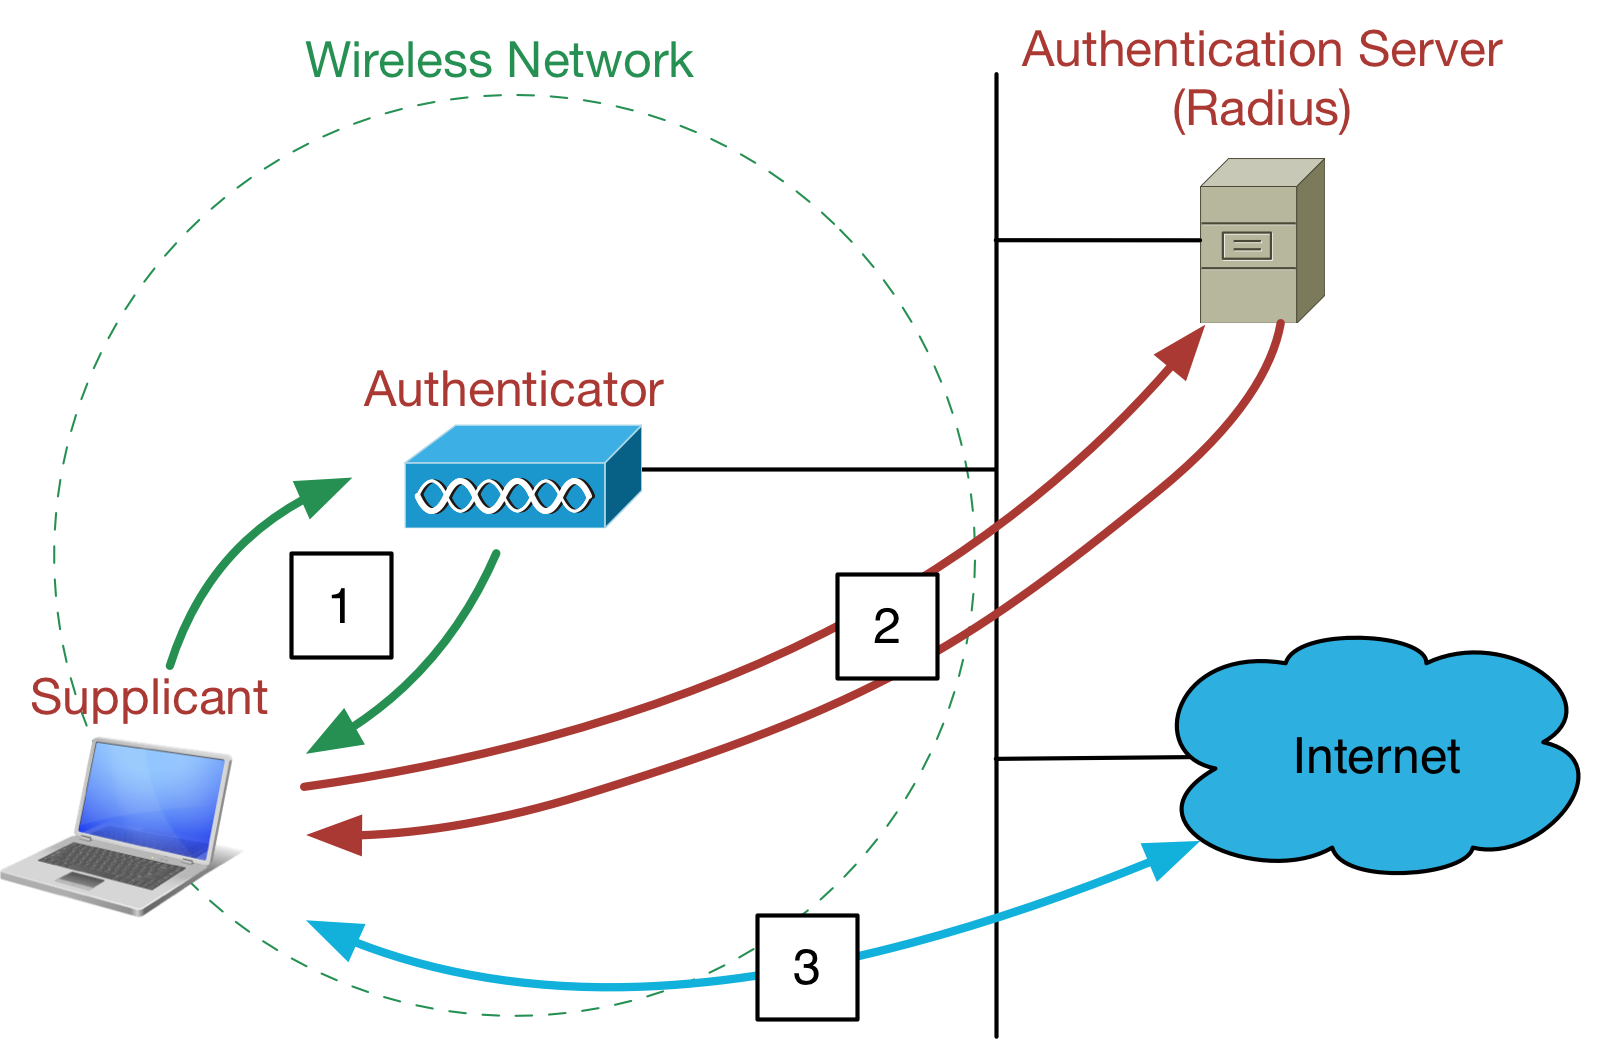
\includegraphics[width=.7\linewidth]{Pictures/chapter2/802.png}
	\caption{\texttt{802.1X} authentication mechanism for WLAN}
	\end{center}
\end{figure}


\subsection{RADIUS}
The Remote Authentication Dial In User Service is defined in \texttt{RFC2865} \cite{rfc2865} and \texttt{RFC2866} \cite{rfc2866}. This is a networking protocol that provides Authentication, Authorization and Accounting (\texttt{AAA}) management for users that connect and use a network service. \texttt{RADIUS} is a client/server protocol that uses \texttt{UDP} for the communications between the \texttt{NAS}\footnote{Network Access Server} and the \texttt{RADIUS} server. It uses port \texttt{1812} for authentication and authorization requests and port \texttt{1813} for accounting requests. The process of granting a supplicant the access to a protected network is divided in three steps.

\begin{description}
	\item[Authentication]: The supplicant sends a connection request to a \texttt{RADIUS} client, called the \texttt{NAS}, in order to get access to a particular network resource. The supplicant credentials (i.e. username and password) are also transmitted by the supplicant to the \texttt{RADIUS} client. Once the client has received the request and credentials, it sends a \texttt{RADIUS} \textit{Access-Request} message to the \texttt{RADIUS} server containing all the authentication information. The server checks if that information is correct by checking that it against a local database or by referring to external sources, such as \texttt{LDAP} servers, to verify the user's credentials. The servers then returns one of the three \texttt{RADIUS} responses to the client:
		\begin{itemize}
			\item \textit{Access-Challenge}: If the \texttt{RADIUS} server needs additional information from the supplicant, it sends this packet to the client requesting that information. The client responds with a new \textit{Access-Request} message. \textit{Access-Challenge} is also used in complex authentication process when a secure tunnel is established between the supplicant and the \texttt{RADIUS} server.

			\item \textit{Access-Accept}: The server grants access to the supplicant.

			\item \textit{Access-Reject}: The server denies access to the supplicant due to identification failure, unknown or inactive user.
		\end{itemize}

	The following figure represents the message exchanges between a \texttt{NAS} and the \texttt{RADIUS} server. The server needs and asks for additional information in the authentication process and finally grant the access to the network.

	\begin{figure}[H]
		\begin{center}
			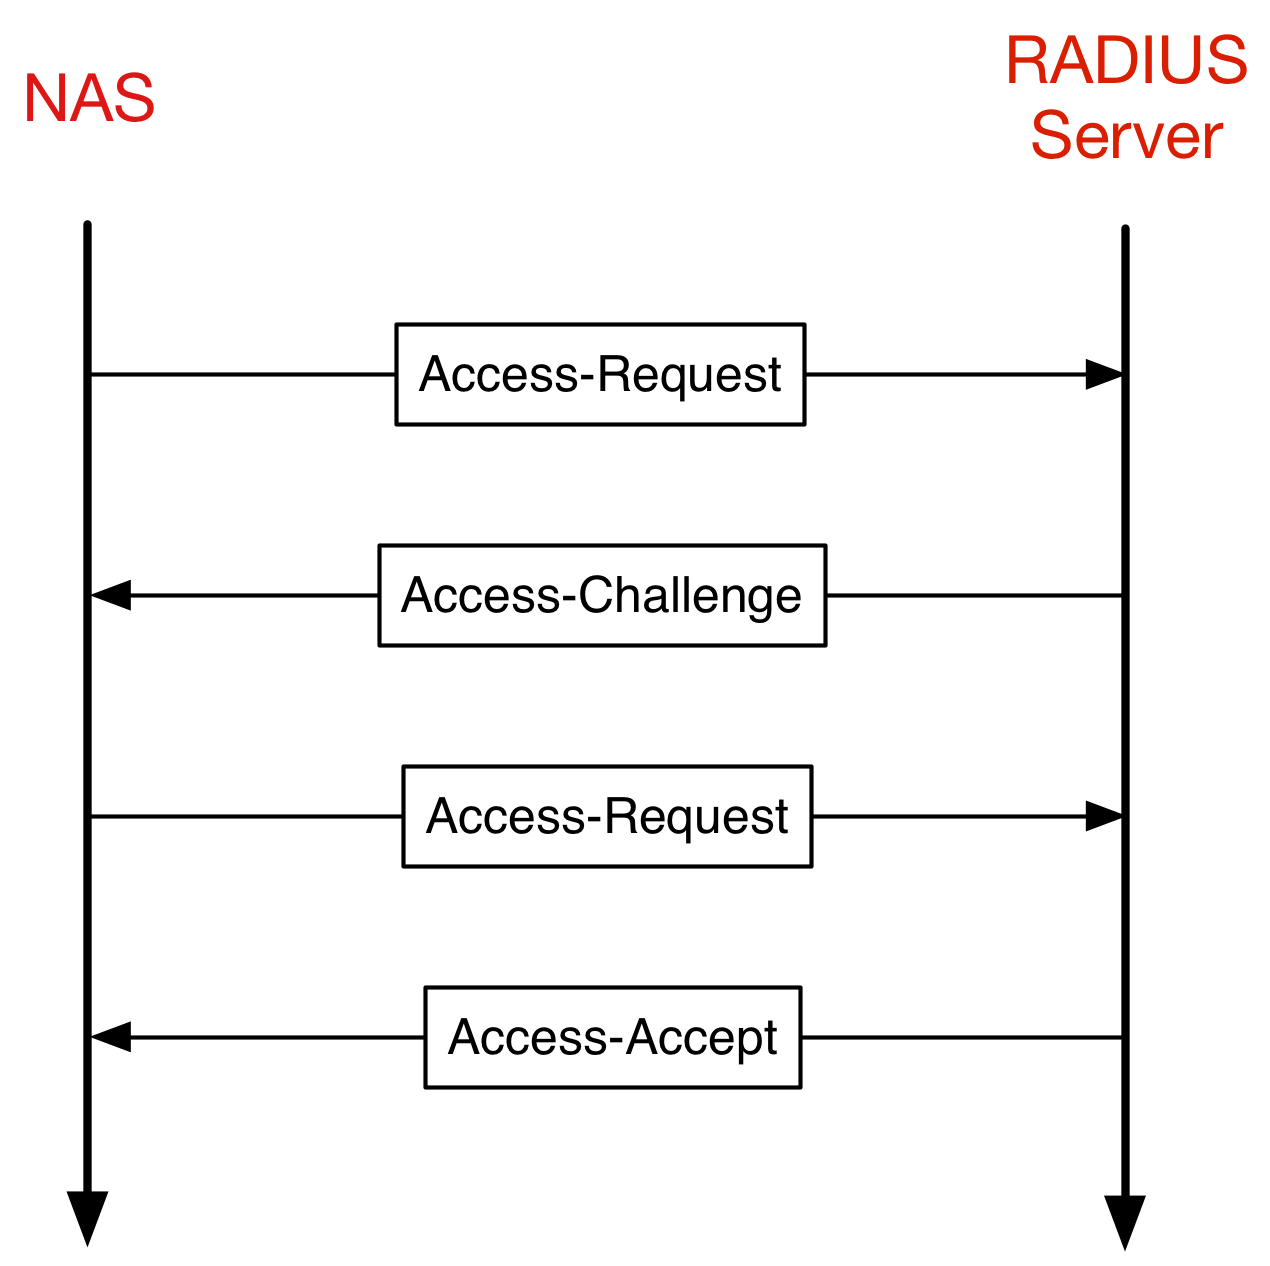
\includegraphics[width=.5\linewidth]{Pictures/chapter2/radius-authentication.png}
			\caption{\texttt{RADIUS} authentication process and message exchanges}
		\end{center}
	\end{figure}
		
	\item[Authorization]: Once \texttt{RADIUS} server has successfully authenticated the user, it can return configuration information to the client (i.e. authorization attributes), stipulating the terms of access to be granted, inside the \textit{Access-Accept} response. Different attributes may be included such as:
		\begin{itemize}
			\item [-] Specific IP address

			\item [-] Maximal length the user may remain connected

			\item [-] \texttt{VLAN} parameters

			\item [-] \texttt{QoS} parameters
		\end{itemize}
	The complete list of possible attributes can be found in \cite{rfc2865}.

	\item[Accounting]: The accounting uses three types of packets, \textit{Accounting Start}, \textit{Interim Update} and \textit{Accounting Stop}. The first packet is transmitted by the \texttt{NAS} to the \texttt{RADIUS} server as soon as the user authentication has succeeded and that he has started to access the network. This packet contains several information about the user such as his username, his affected IP address, the date of connection, and so on. The last packet is sent when the user disconnects from the network. Upon reception of that \textit{Accounting Stop} packet, the sever can end the user's session and log all the information about that particular session. The \textit{Interim Update} packet is sent by the \texttt{NAS} to update the information of the current session. All these packets are encapsulated inside an \textit{Accounting-Request} \texttt{RADIUS} message. The server responds with a \textit{Accounting-Response} message. The purpose of the accounting is to keep a trace of everything that happens on the network and to keep data about all the users that have accessed it. Plus it is also used for statistical analysis and network monitoring.

	The following figure depicts the accounting messages flow between the \texttt{NAS} and the \texttt{RADIUS} server. On packet of each type is represented to get a better overview.

	\begin{figure}[H]
		\begin{center}
			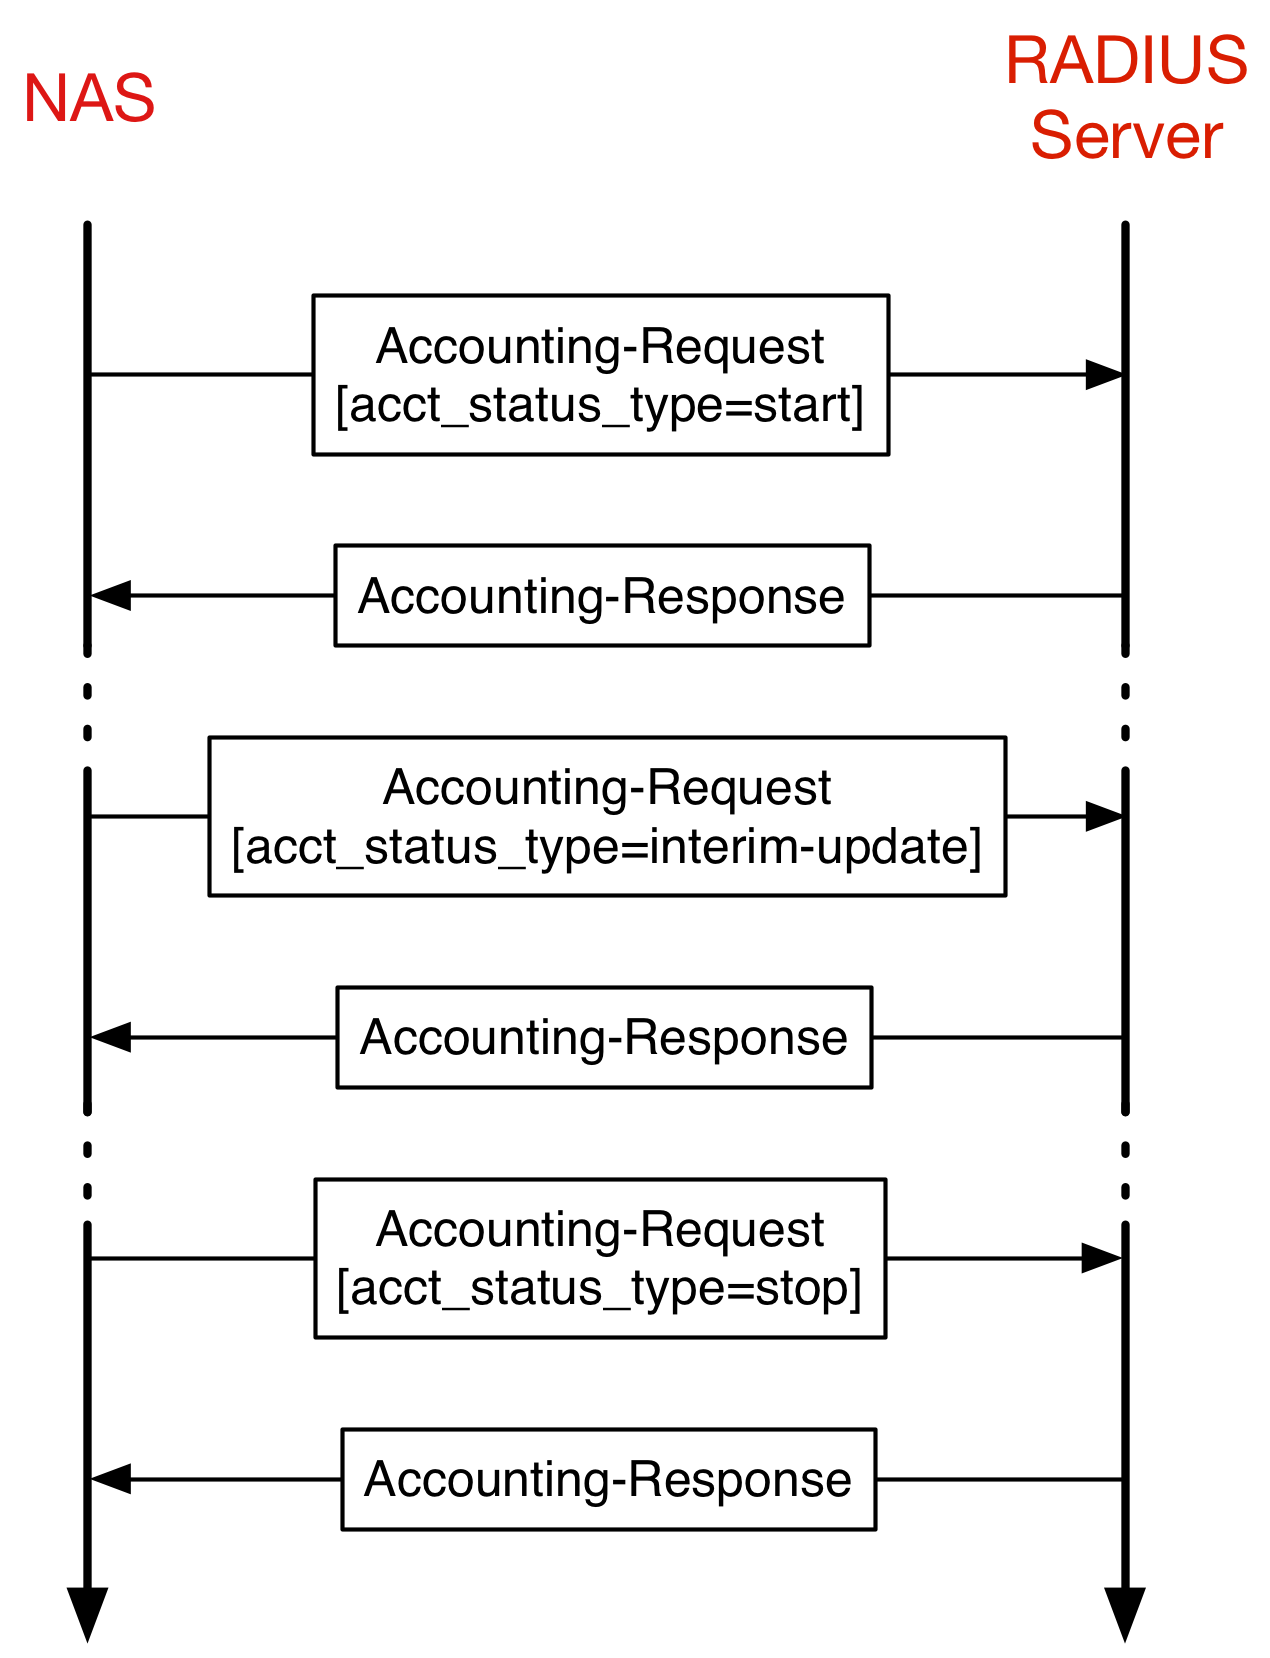
\includegraphics[width=.5\linewidth]{Pictures/chapter2/radius-accounting.png}
			\caption{\texttt{RADIUS} accounting messages flow}
		\end{center}
	\end{figure}


\end{description}


\subsection{WiSM}
Cisco Wireless Services Module 2 (WiSM2)\\
TODO

\subsection{SNMP}

The Simple Network Management Protocol is an application layer protocol that facilitates the exchange of management information between network devices \cite{snmp}. It is part of the TCP/IP protocol suite and it is mainly used by network administrators to get information about devices on the network and the network performances. These information help the administrators to resolve problems on the network or simply to manage it.
A SNMP network has three main components:

\begin{itemize}
	\item \texttt{Network-management system (NMS)}: A NMS is the main component of an SNMP-managed network. It is the management entity that controls the managed devices. It uses the SNMP protocol and can interact with the managed devices to get information using special commands and messages.
	
	\item \texttt{Managed devices}: It is a network device that contains an SNMP agent. They collect and store information to make them available for the network-management systems. Those devices can be routers, servers, switches, etc. They also run the SNMP protocols to be able to respond to the requests made by the NMS.
	
	\item \texttt{Agents}: An agent is the thinking part of a managed device. It is a software module that understands the management information and translates them into a SNMP compatible form.
\end{itemize}

\begin{figure}[H]
\centering
	\includegraphics[width=.7\linewidth]{Pictures/chapter2/snmp.png}
	\caption{A typical SNMP managed network}
\end{figure}

All the network objects are described and organized hierarchically in a Management Information Base (MIB). There are MIBs for each set of related network entities that can be managed. These MIBs are accessed using a network-management protocol such as SNMP.



\section{WLAN authentication process}
Let's analyze the authentication process mechanism with a WLAN network.
As explained before, with the \texttt{IEEE 802.1X} standard, there are two key parts, the \textit{Authenticator} and the \textit{Authentication Server}. In the case of a WiFi authentication process, a third one can be added to this list and is called the \textit{Supplicant}. The supplicant is simply the wireless client that asks for an authentication in order to have access to the protected network. The authentication process works in several key steps and uses different protocols.

First of all, the supplicant who wants to access the network needs to make a special request to the authenticator. During that step the protocols that are used between the supplicant and the authenticator are a combination of \texttt{802.1X} and \texttt{EAP} protocol (\textit{Extensible Authentication Protocol}). Thanks to \texttt{802.1X} protocol, the authenticator can refuse any access to the network as long as the authentication server has not authenticated the client and accepted to open the access (i.e. open the port). The \texttt{EAP} defines a standard for the messages that are going to be exchanged between the supplicant and the authentication server. It is a  transport protocol for the authentication protocols. Those \texttt{EAP} messages are encapsulated over \texttt{IEEE 802} and this encapsulation is known as \texttt{EAPOL} (for \textit{"EAP over LAN"}. Technically we should say \texttt{EAPOW} for a wireless network but it is only to refer to an \texttt{EAPOL} message that is being sent using \texttt{802.11} wireless network transmission and the standard never mention \texttt{EAPOW}).

\texttt{EAP} provides several authentication methods. The \texttt{EAP} methods that are used within the UCL's WLAN  security management are either \texttt{EAP-TTLS} (\textit{EAP-Tunneled Transport Layer Security}) or \texttt{EAP-PEAP} (\textit{Protected Extensible Authentication Protocol}) chosen by the OS. They both are an authentication protocol that rely on an encrypted and secured tunnel. With the \texttt{TTLS} method, the client is authenticated with his username and password and the server is authenticated with a \texttt{X.509} certificate. When the client starts an authentication process, he uses the server certificate to encrypt all the messages he is going to send to the authentication server. In other words, this certificate is used as a key for encrypting the communication between the supplicant and the authentication server. It is also used to authenticate the authentication server (i.e. to verify that the server the client is talking to is really the UCL's server that authenticate the clients).


Second, once the authenticator has received the request from the supplicant, he has to forward it to the authentication server. The protocol used between the authenticator and the authentication server is the \texttt{RADIUS} protocol. All the requests made by the supplicant, in \texttt{802.1X/EAP} messages, are translated into \texttt{RADIUS} and forwarded to the authentication server. This is know as the \texttt{EAP over RADIUS} protocol.The authenticator server then grants the access or not to the client and sends back a response to the authenticator telling it to open the network access to the client.

As seen on the following picture of the UCL's wireless network topology, the supplicant sends (1) its information to the authenticator (composed of the access point and the WiFi controller) in \texttt{EAP} frames. The authenticator then forwards (2) them in \texttt{RADIUS} encapsulated packets to the authentication server. After queries on the \texttt{LDAP} databases (2) and exchanges with the authenticator, the server sends back (3) a packet saying if the supplicant can access or not to the network. If so, the supplicant is authenticated but still needs an IP address to access the Internet. In order to do so, it asks the \texttt{DHCP} server (4). Once it got its address from the server it can fully access the Internet (5).

fully authenticated and can use (4) the protected network.

\begin{figure}[H]
	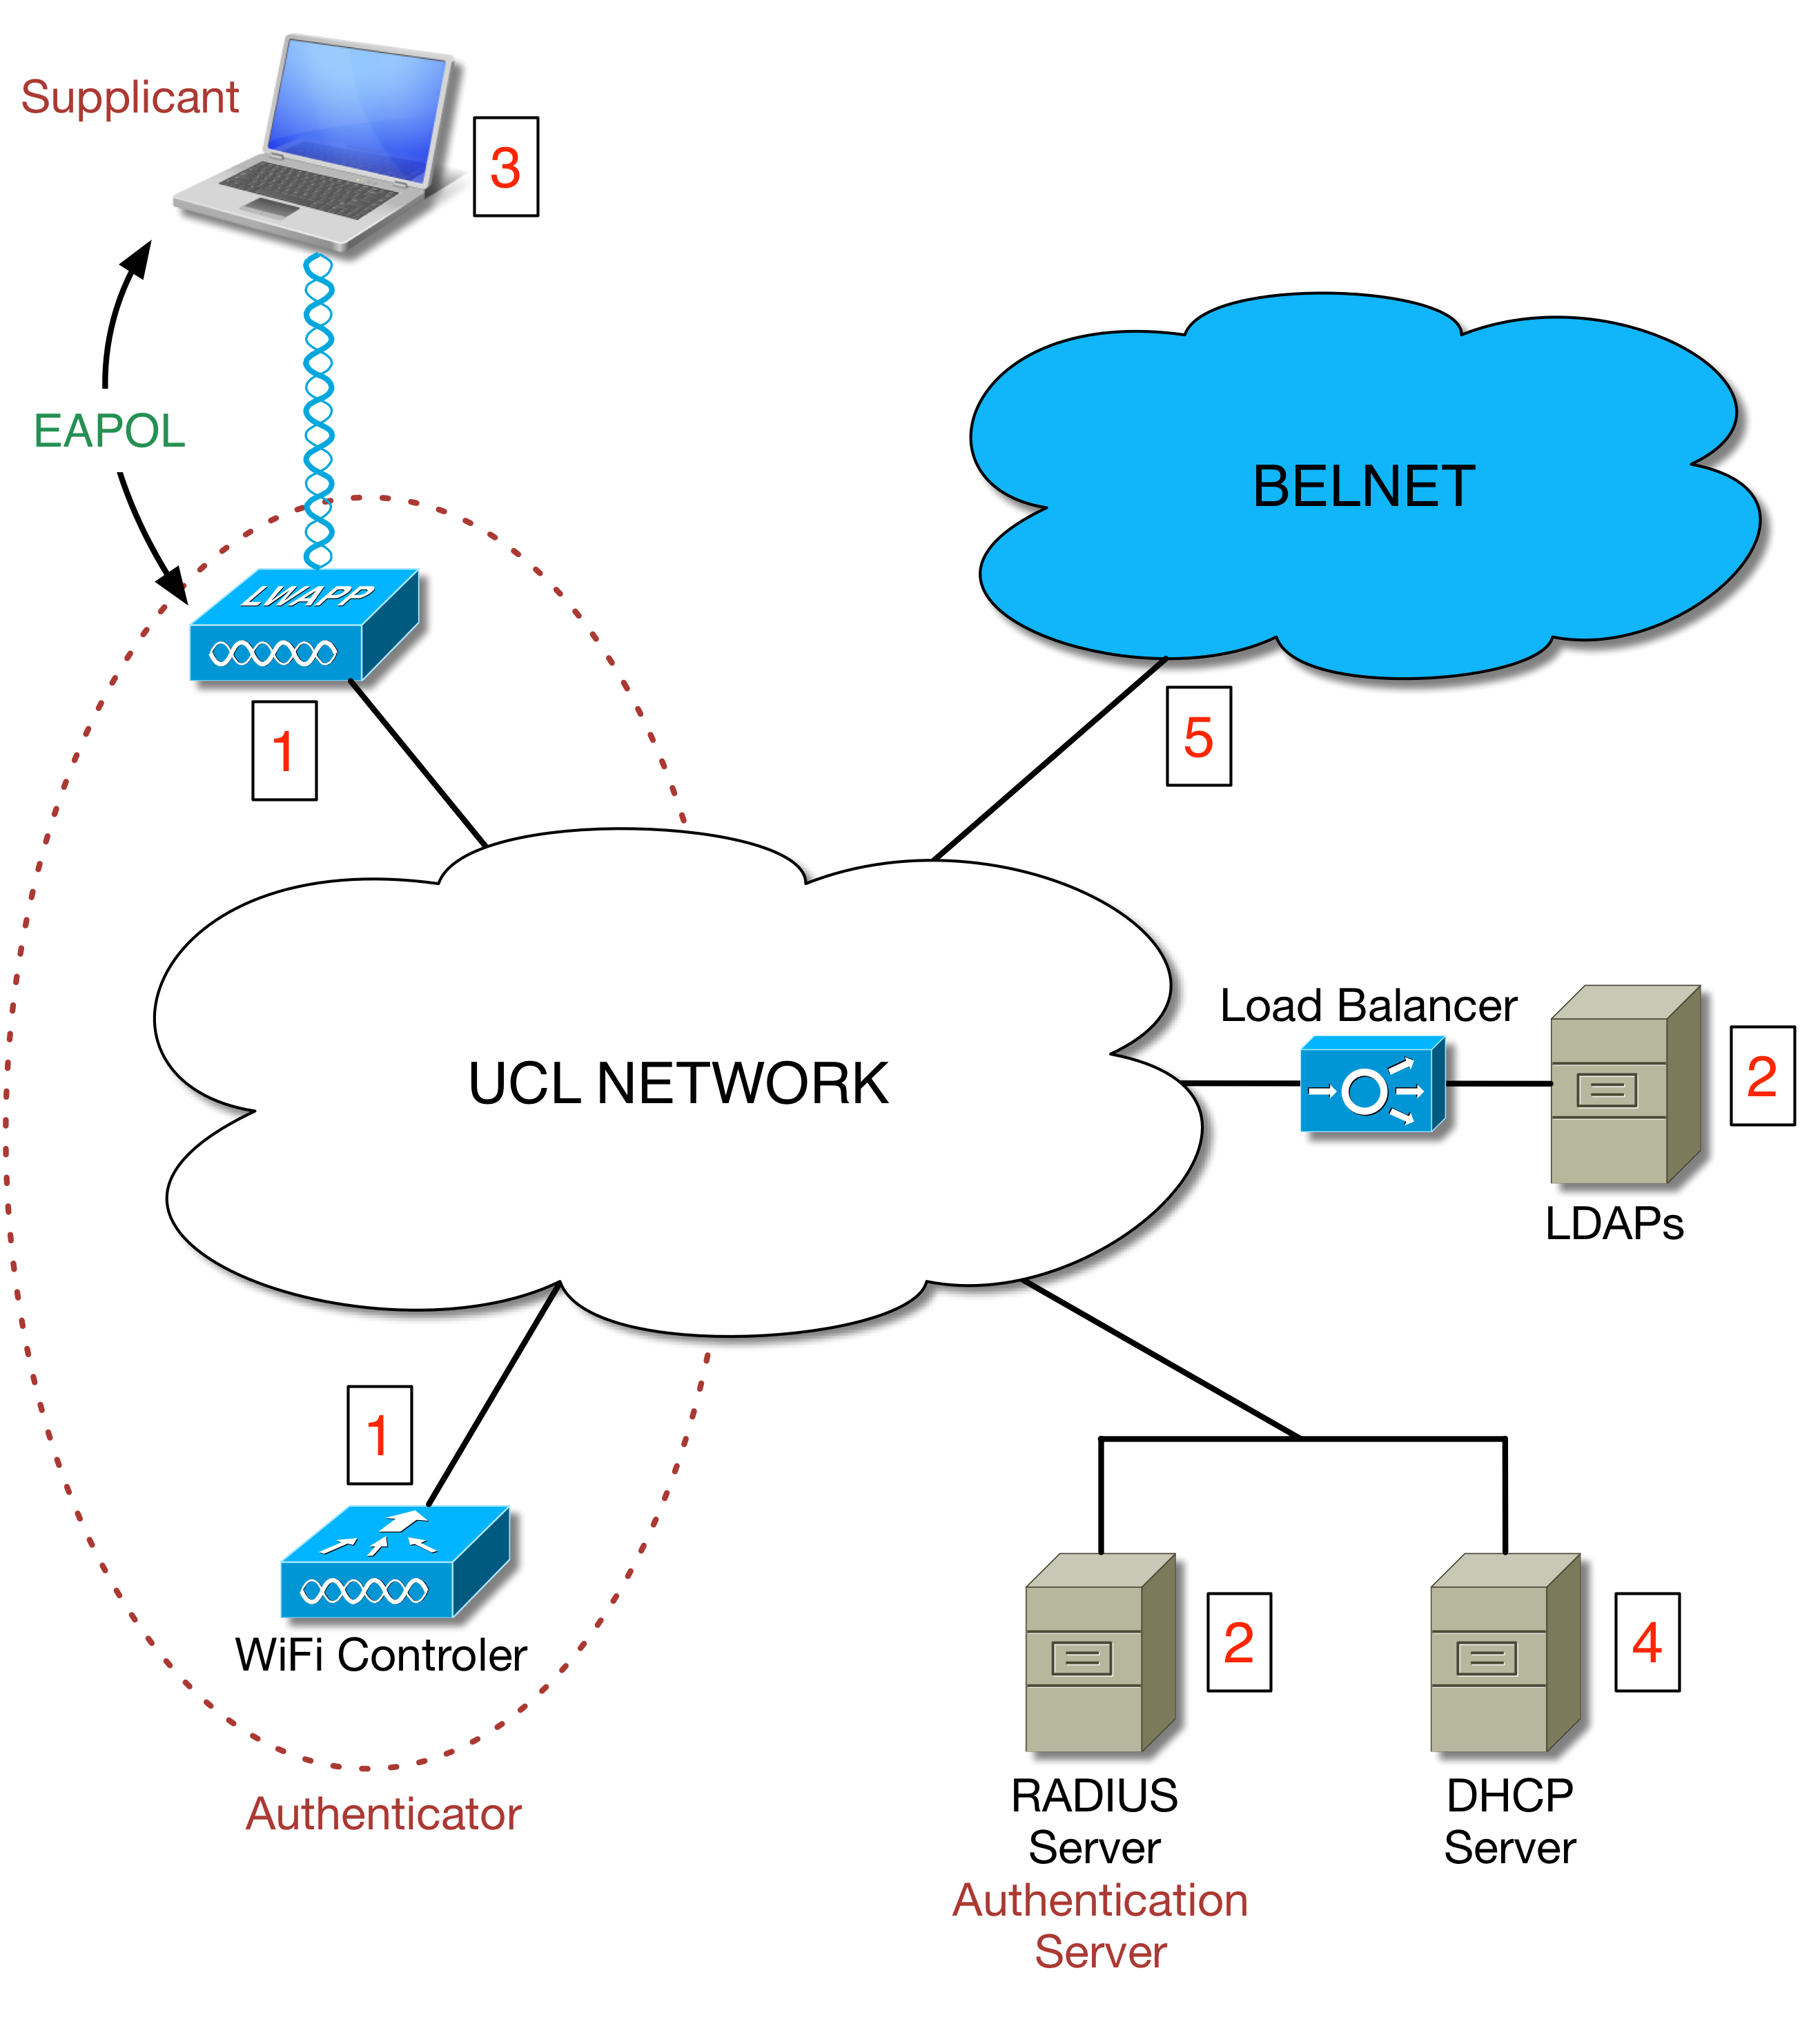
\includegraphics[width=.9\linewidth]{Pictures/chapter2/topology2.png}
	\caption{Authentication process on a UCL's WLANs}
\end{figure}


\subsection{student.UCLouvain authentication example}
To illustrate how the whole authentication process works, let's take a closer look to what happens when a student wants to connect to the \texttt{student.UCLouvain} network.
As detailed above, this network is protected by the \texttt{802.1X} authentication protocol. Thus the client first needs to authenticate himself before being able to access the Internet.
As a reminder, the client who wants to connect the network is called the \textit{supplicant}. This supplicant is going to first make a standard \texttt{802.11} association with the authenticator using \texttt{WPA/WPA2}. The authenticator is composed of the access point to which the supplicant is trying to connect and the WLAN controller that is going to handle the whole authentication request. Once this association has been made, the authenticator understands that the supplicant wants to get an access to the protected network and thus a \texttt{802.1X} session between them is started. At this state, only \texttt{802.1X} traffic is allowed (i.e. only \texttt{EAP} messages are accepted during the transmissions).

The first message the supplicant is going to send to the authenticator is an \texttt{EAPOL-Start} frame in order to initiate the authentication process. When the authenticator receives that frame, it sends an \texttt{EAP-Request Identity} frame to the supplicant that answers with an \texttt{EAP-Response Identity} frame containing the supplicant's identity. The authenticator encapsulates this response in a \texttt{RADIUS Access-Request} packet and forwards it to the authenticator server.

Once the authentication server has received that packet it sends a \texttt{RADIUS Access Challenge} back to the authenticator containing an \texttt{EAP Request} specifying the type of \texttt{EAP} method to use (\texttt{TTLS} or \texttt{PEAP}) in order to validate the identity of the supplicant and to specify how the credentials are submitted. The authentication server also sends its certificate during that negotiation. The authenticator encapsulates that \texttt{EAP Request} in an \texttt{EAPOL} frame and sends it to the supplicant.

Since the supplicant has a copy of the server certificate, it can checks if the one received during the negotiation is the same in order to authenticate the server's identity. Once its identity has been proved, the supplicant builds a \texttt{TLS-encrypted} tunnel with the authentication server. It then sends its credential securely inside this channel.

The authentication server validates the username and password of the supplicant and sends back a \texttt{RADIUS Access-Accept} packet to the authenticator that sends an \texttt{EAP-Success} frame to the supplicant. The authenticator opens the port for the supplicant and by doing so, completing the process of authentication and allowing the user to access the Internet after having negotiated a \texttt{WPA/WPA2} key with the authenticator in order to encrypt the further transmissions.

The following figure represents the main steps of the authentication process for the \texttt{student.UCLouvain} network:

\begin{figure}[H]
	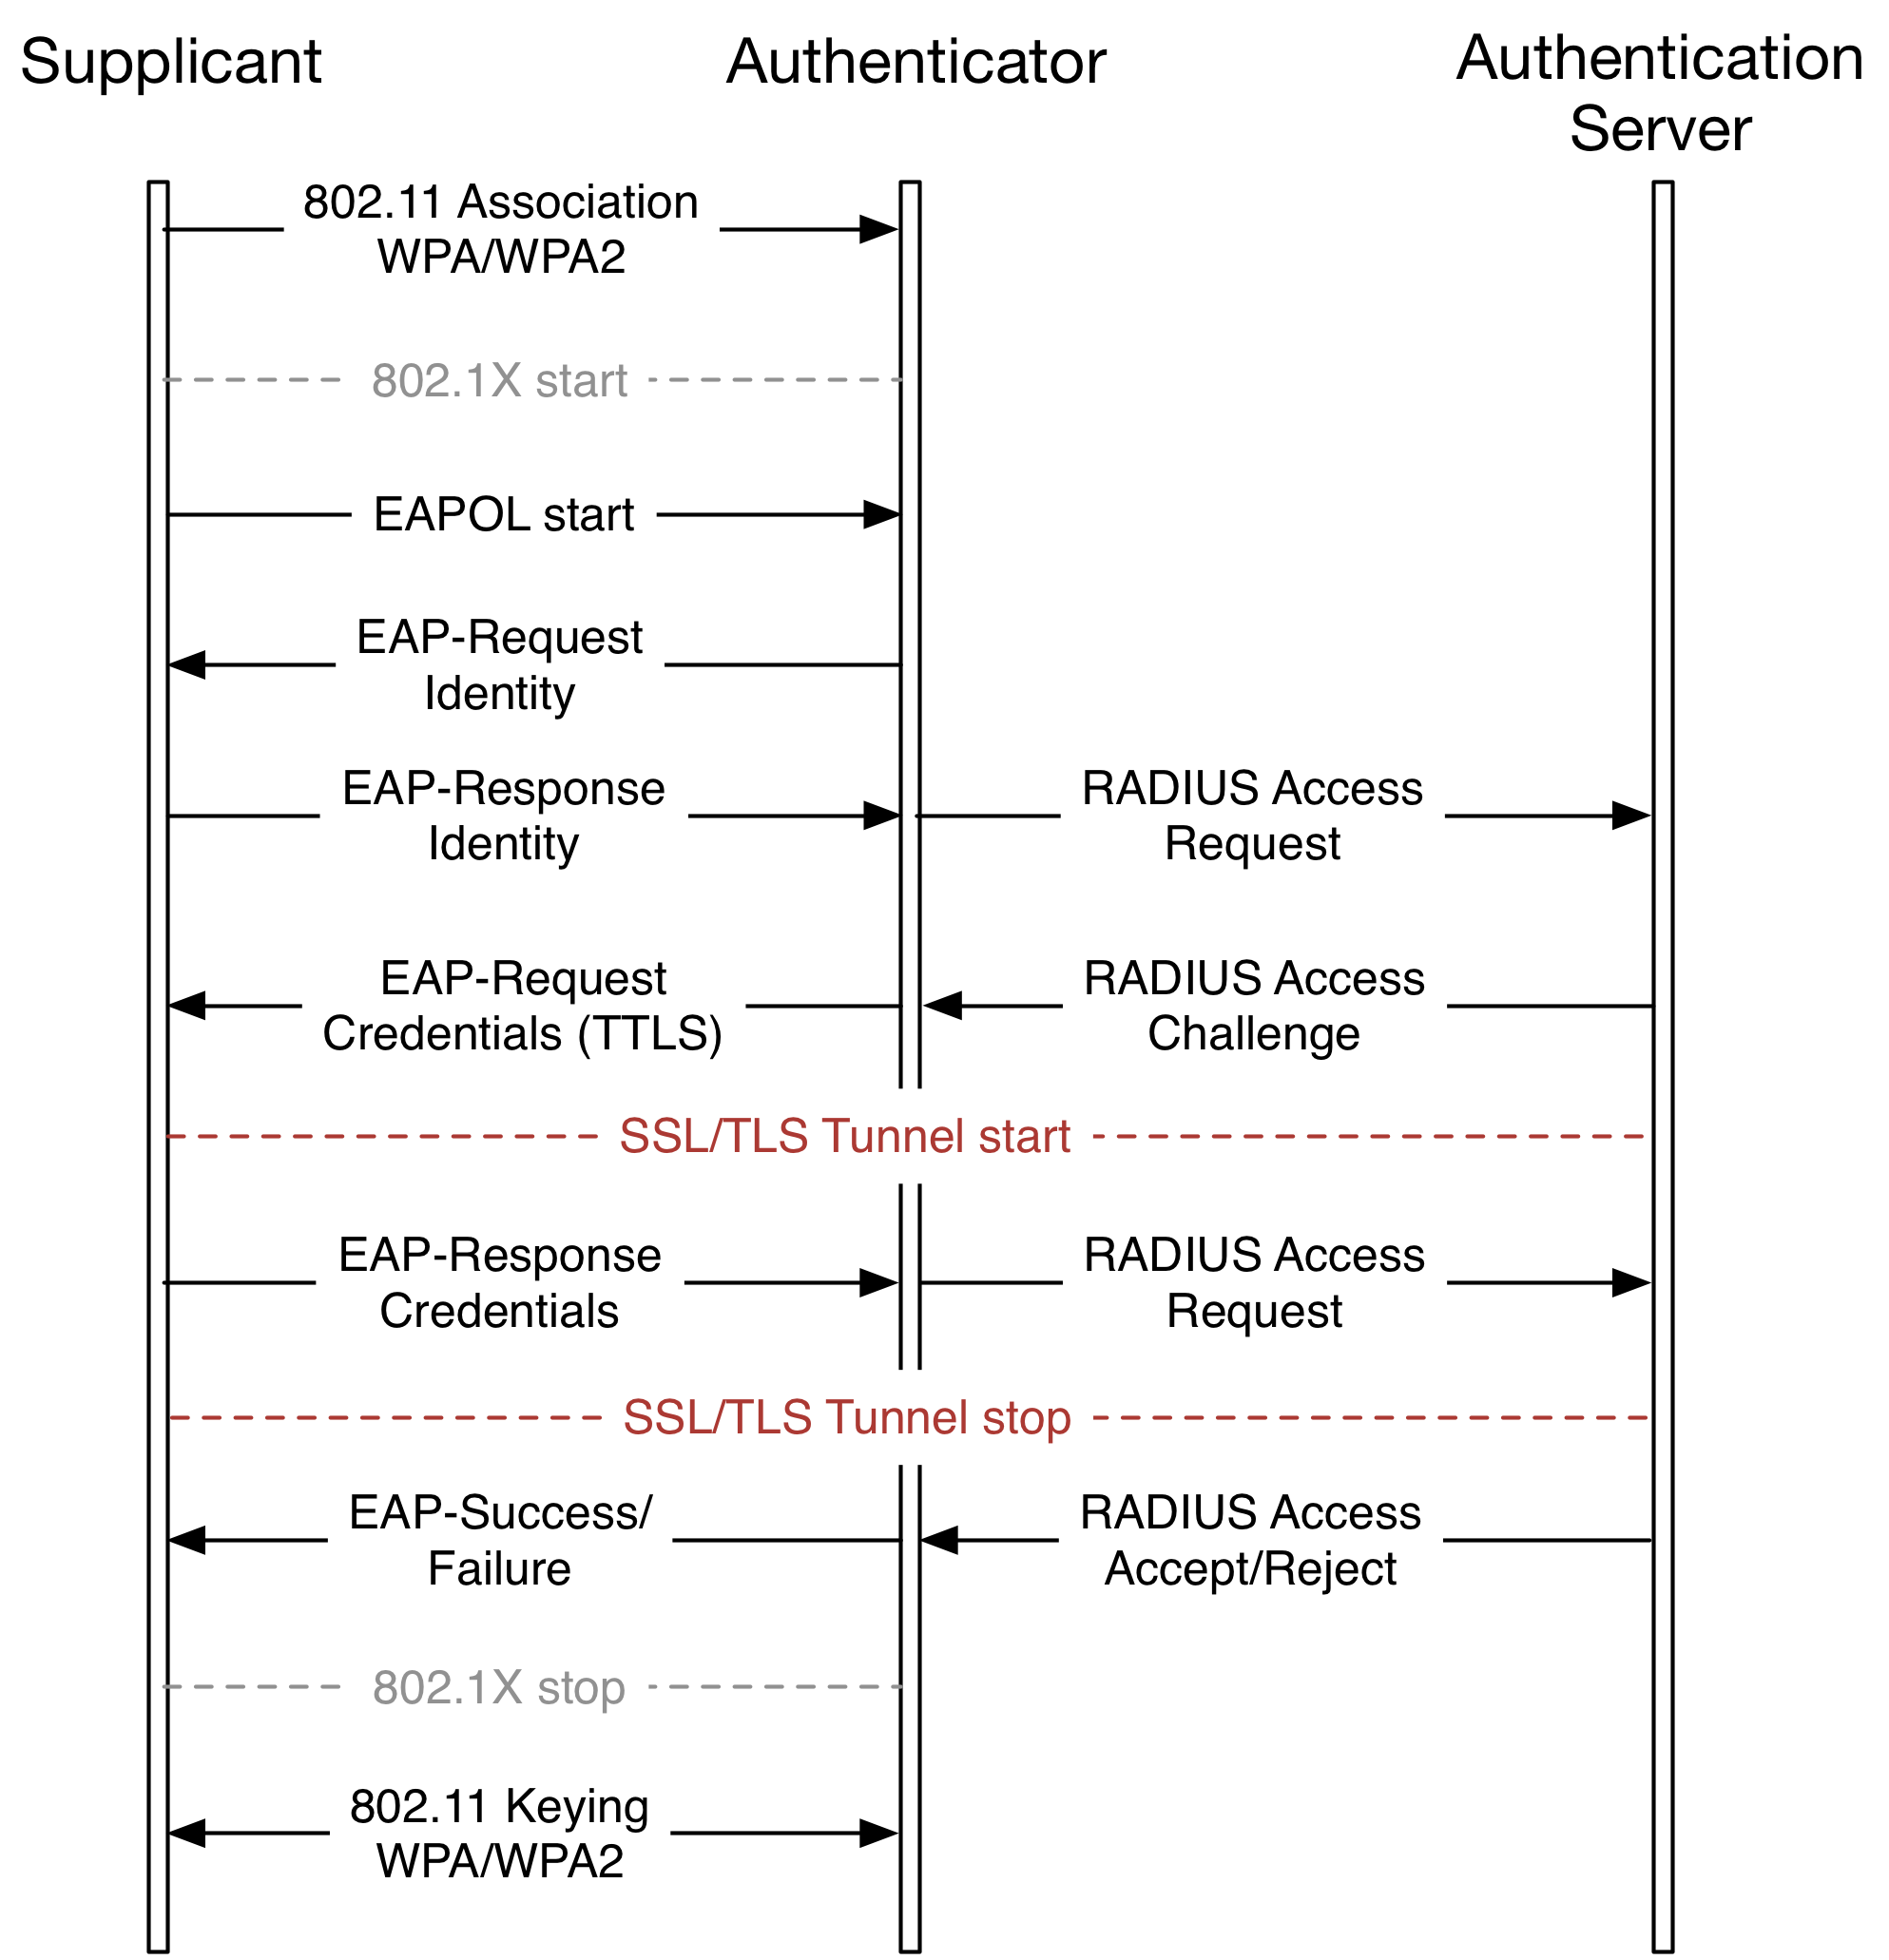
\includegraphics[width=.9\linewidth]{Pictures/chapter2/student.png}
	\caption{student.UCLouvain authentication process}
\end{figure}


\subsection{eduroam authentication example}
Let's take another WLAN authentication process example with the \texttt{eduroam} network which is a bit different than the example seen before.
As explained in \cite{eduroamRadius}, the \texttt{eduroam} project is "\textit{A wolrdwide federation of} \texttt{RADIUS} \textit{ servers facilitating network access for roaming academic affiliates using} \texttt{IEEE 802.1X} \textit{as the vehicle. eduroam's use of} \texttt{802.1X} \textit{in concert with} \texttt{RADIUS} \textit{means the network is built around well understood, established, and easy to manage standards which are often already deployed within the network infrastructure of educational institutions}".

Since \texttt{eduroam} is also using the \texttt{802.1X}, when a client wants to connect to the network, he is not able to pass any traffic other than \texttt{802.1X} until his request is accepted by the authentication server. As for the \texttt{student.UCLouvain} network, the communication between the supplicant and the authenticator also involves \texttt{EAP} conversation.The supplicant sends its \texttt{EAP} messages to the authenticator that forwards them to the authentication server in the form of a \texttt{RADIUS} request. To ensure the protection of the credentials and information sent during the authentication negotiation, eduroam uses either \texttt{TTLS} or \texttt{PEAP} (\textit{Protected Extensible Authentication Protocol}).A \texttt{TLS-encrypted} tunnel is also created between the supplicant and the authentication server.

As a student from another university than the Catholic University of Louvain can access and connect to the \texttt{eduroam} network from inside the Louvain-la-Neuve campus, the local authentication server, in Louvain-la-Neuve, is not the one that is going to handle the authentication request. Indeed, if the user comes from the University of Seville in Spain, for example, its authentication request within the UCL's campus is first handled by the local \texttt{RADIUS} server. This server forwards the request to the Belnet \texttt{RADIUS} server since it does not know the realm used by the Spanish student. That Belnet server understands that this student is not from Belgium. It thus forwards the request to the European \texttt{RADIUS} server, Terena. Terena understands that the user comes from Spain so it forwards the request to the Spanish national \texttt{RADIUS} server that finally forwards the request to the University of Seville's server. The response takes the same route to get to Louvain-la-Neuve.

The \texttt{RADIUS} protocol supports that forwarding in its proxy mode. To prevent any administrators not responsible for the handling of the authentication request, the \texttt{TLS-encrypted} tunnel is propagated throughout the \texttt{RADIUS} infrastructure. Thanks to that tunnel, the intermediate authenticator does not handle sensitive information during the authentication process.

Here is a representation of the authentication request communications between the supplicant, the authenticator and the authentication server with \texttt{RADIUS} proxying:
\begin{figure}[H]
	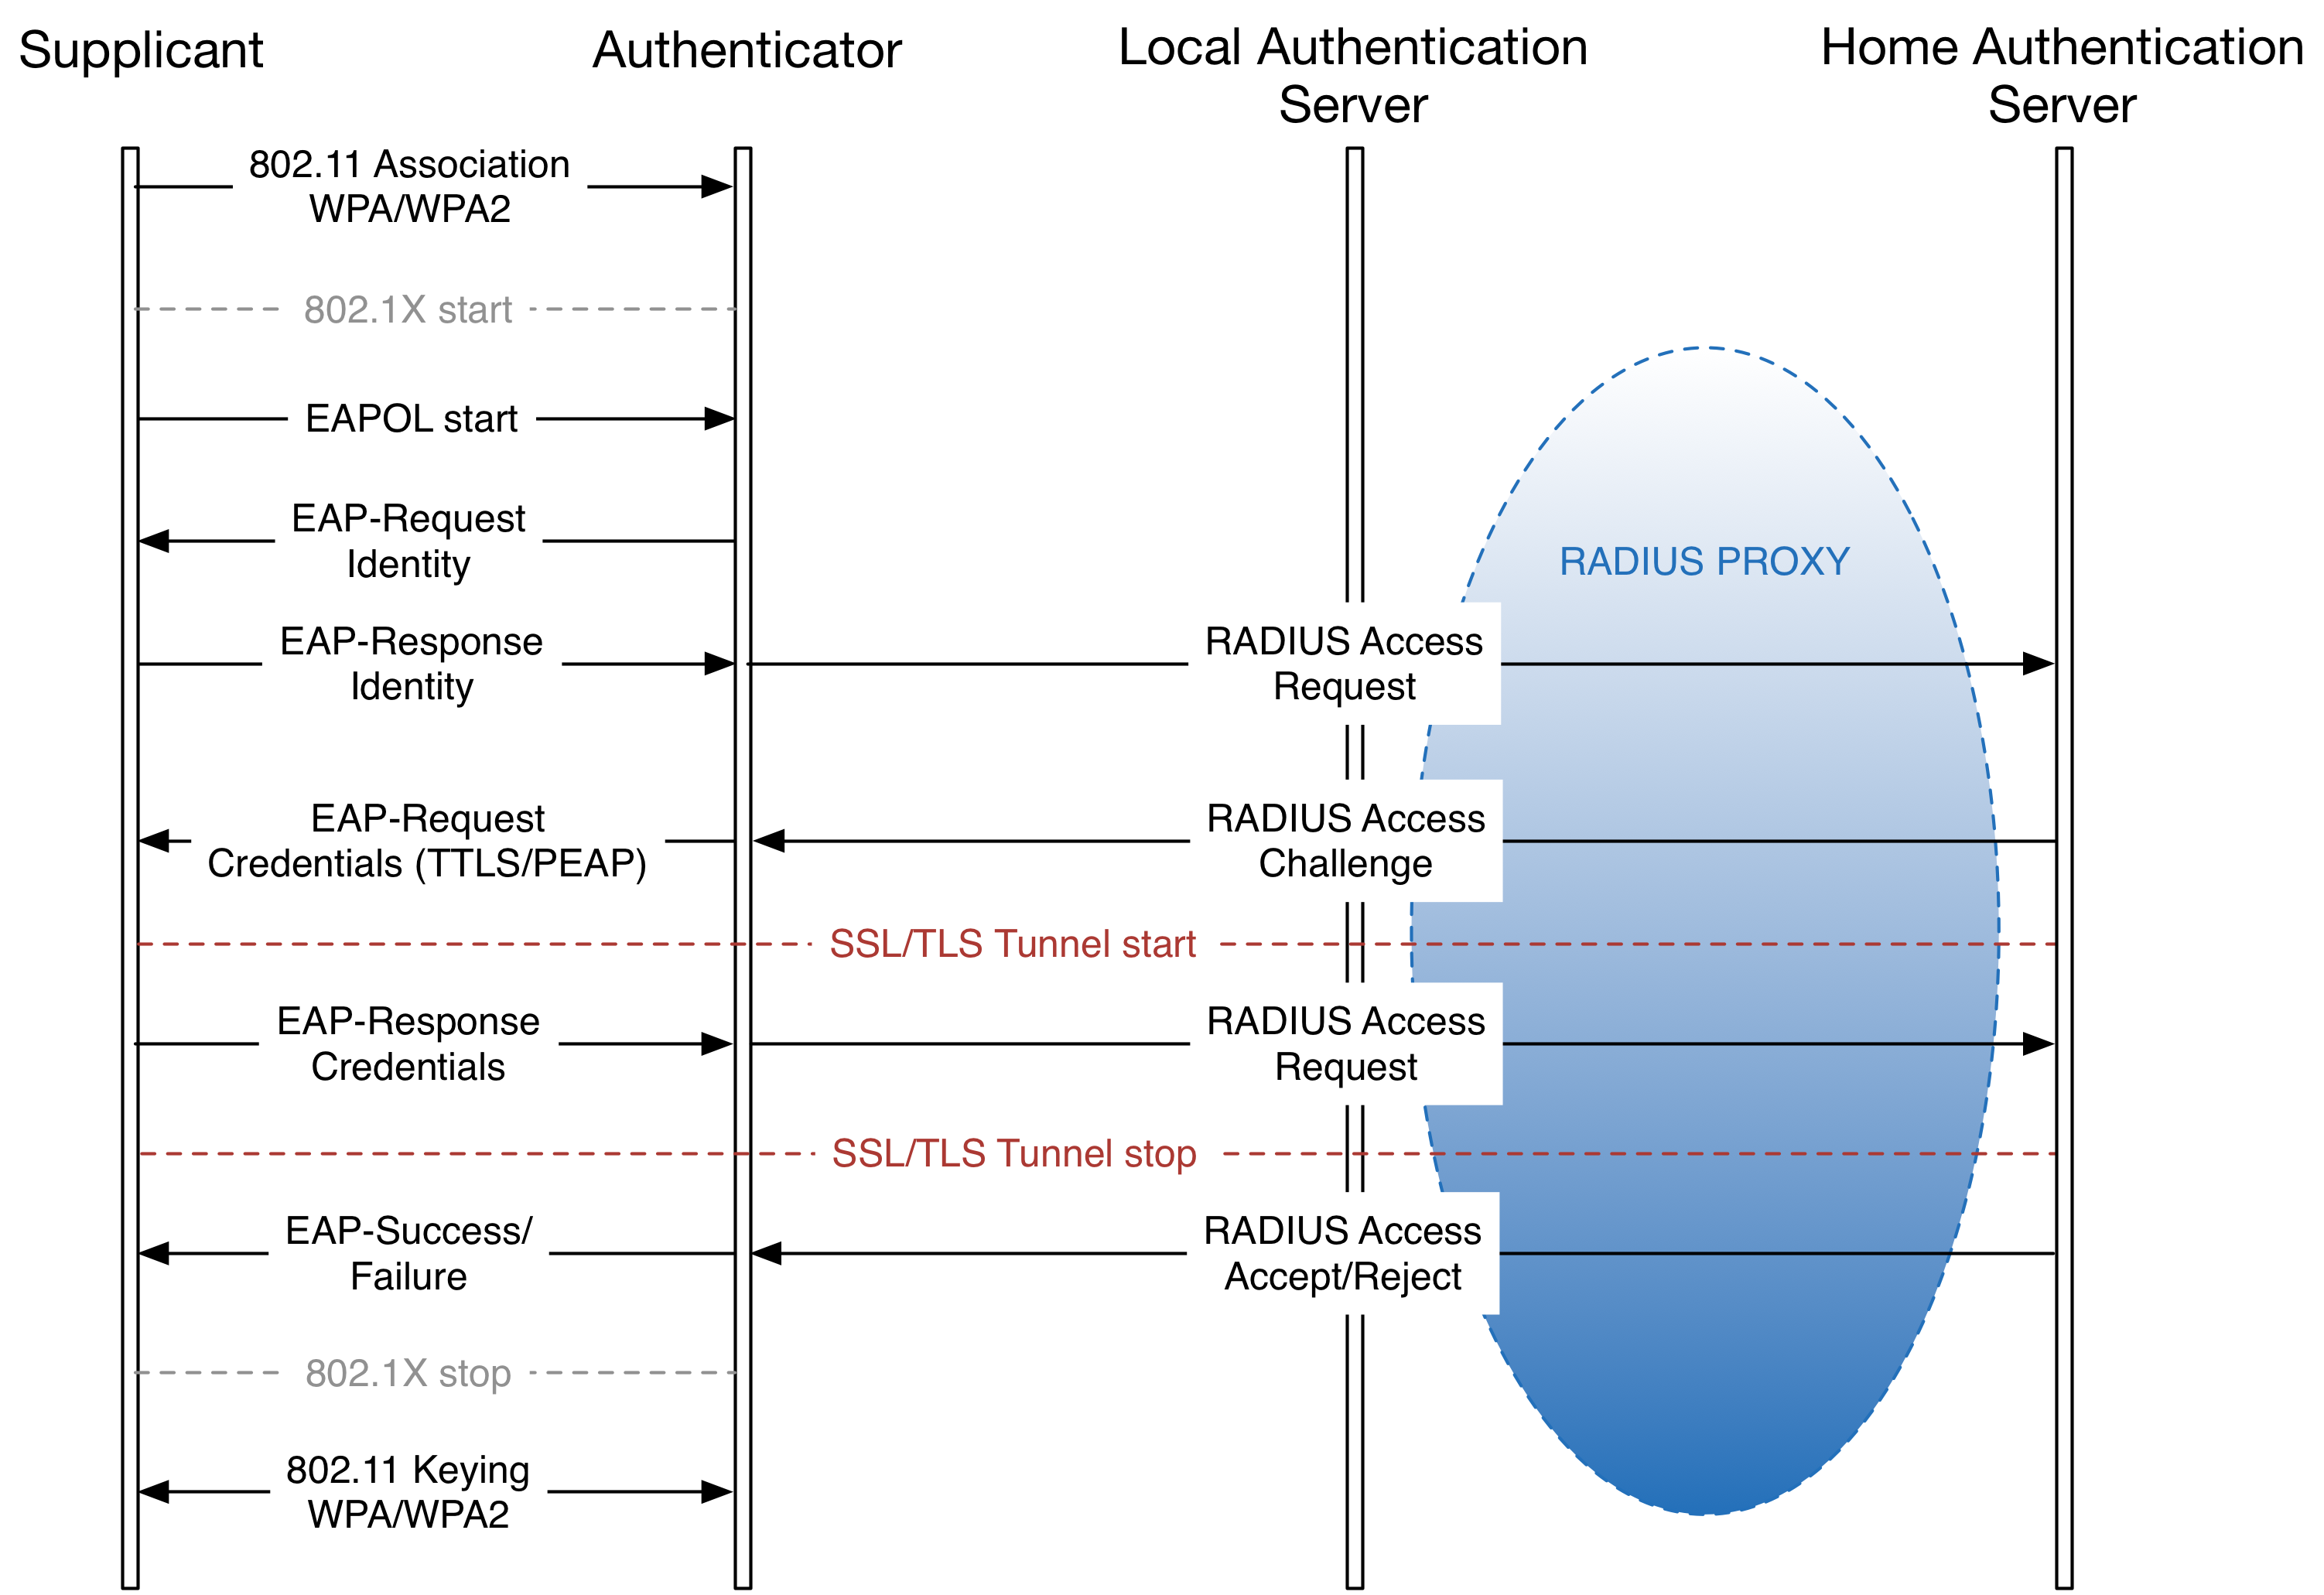
\includegraphics[width=1\linewidth]{Pictures/chapter2/eduroam1.png}
	\caption{eduroam authentication process}
\end{figure}

\section{Infrastructure architecture}
Within the Catholic University of Louvain's network infrastructure architecture, the Internet access is provided by Belnet via a 10Gbit Ethernet link. This link is connected to one of the seven \textit{neighborhood routers} called \texttt{CtPythagore}. There is also a second 1Gbit Ethernet link connected to another neighborhood router called \texttt{CtHalles}. This second link is never used and is, in fact, a backup link in case of a failure of the main one.

The other neighborhood routers are \texttt{CtLew}, \texttt{CtStevin}, \texttt{CtCarnoy}, \texttt{CtMichotte} and \texttt{CtSHI1C}. They are all on the Louvain-la-Neuve campus expect for \texttt{CtLew} that lies on the Woluwe campus in Brussels. Those neighborhood routers are all \texttt{Cisco Catalyst 6509} switches and are the campus core routers. Two of them (\texttt{CtSH1C} and \texttt{CtMichotte}) include a \texttt{Cisco WiSM2} (\textit{Wireless Services Module 2}) controller. The infrastructure also contains two data centers called \texttt{CtTier2} and \texttt{CtAquarium}. Each one of those data center has a load balancer. The two \texttt{DHCP} servers as well as the \texttt{LDAP} servers are located behind those load balancers.

Here is a representation of the UCL's network infrastructure.

\begin{figure}[H]
	
\includegraphics[width=1\linewidth]{Pictures/chapter2/ucl.png}
	\caption{UCL's network infrastructure architecture}
\end{figure}


Each building on the Louvain-la-Neuve campus has a direct connectivity with the network. Inside there are several access points (there are approximatively 300 access points on the Louvain-la-Neuve's campus and most of them are \texttt{Cisco AIR-AP1242AG}. Yet they are starting to be replaced, only in the INGI buildings for this moment, by either \texttt{Cisco Aironet 3600} or \texttt{Cisco Aironet 3700}) that provide an Internet access to the clients. Each access point is connected to a switch \texttt{Cisco Catalyst 2960-48LPS}. This switch only has 48 ports so there are several one of them, in each building, place in a patch room. Those switches are connected to another switch \texttt{Cisco Catalyst 2960G-24TC-L} that has a direct fiber connection with one of the seven neighborhood routers. Thanks to that connection, each building is connected to the UCL network and thus, to the WiFi controller.

The following figure represents a simplified overview of how the buildings are connected to the network.

\begin{figure}[H]
	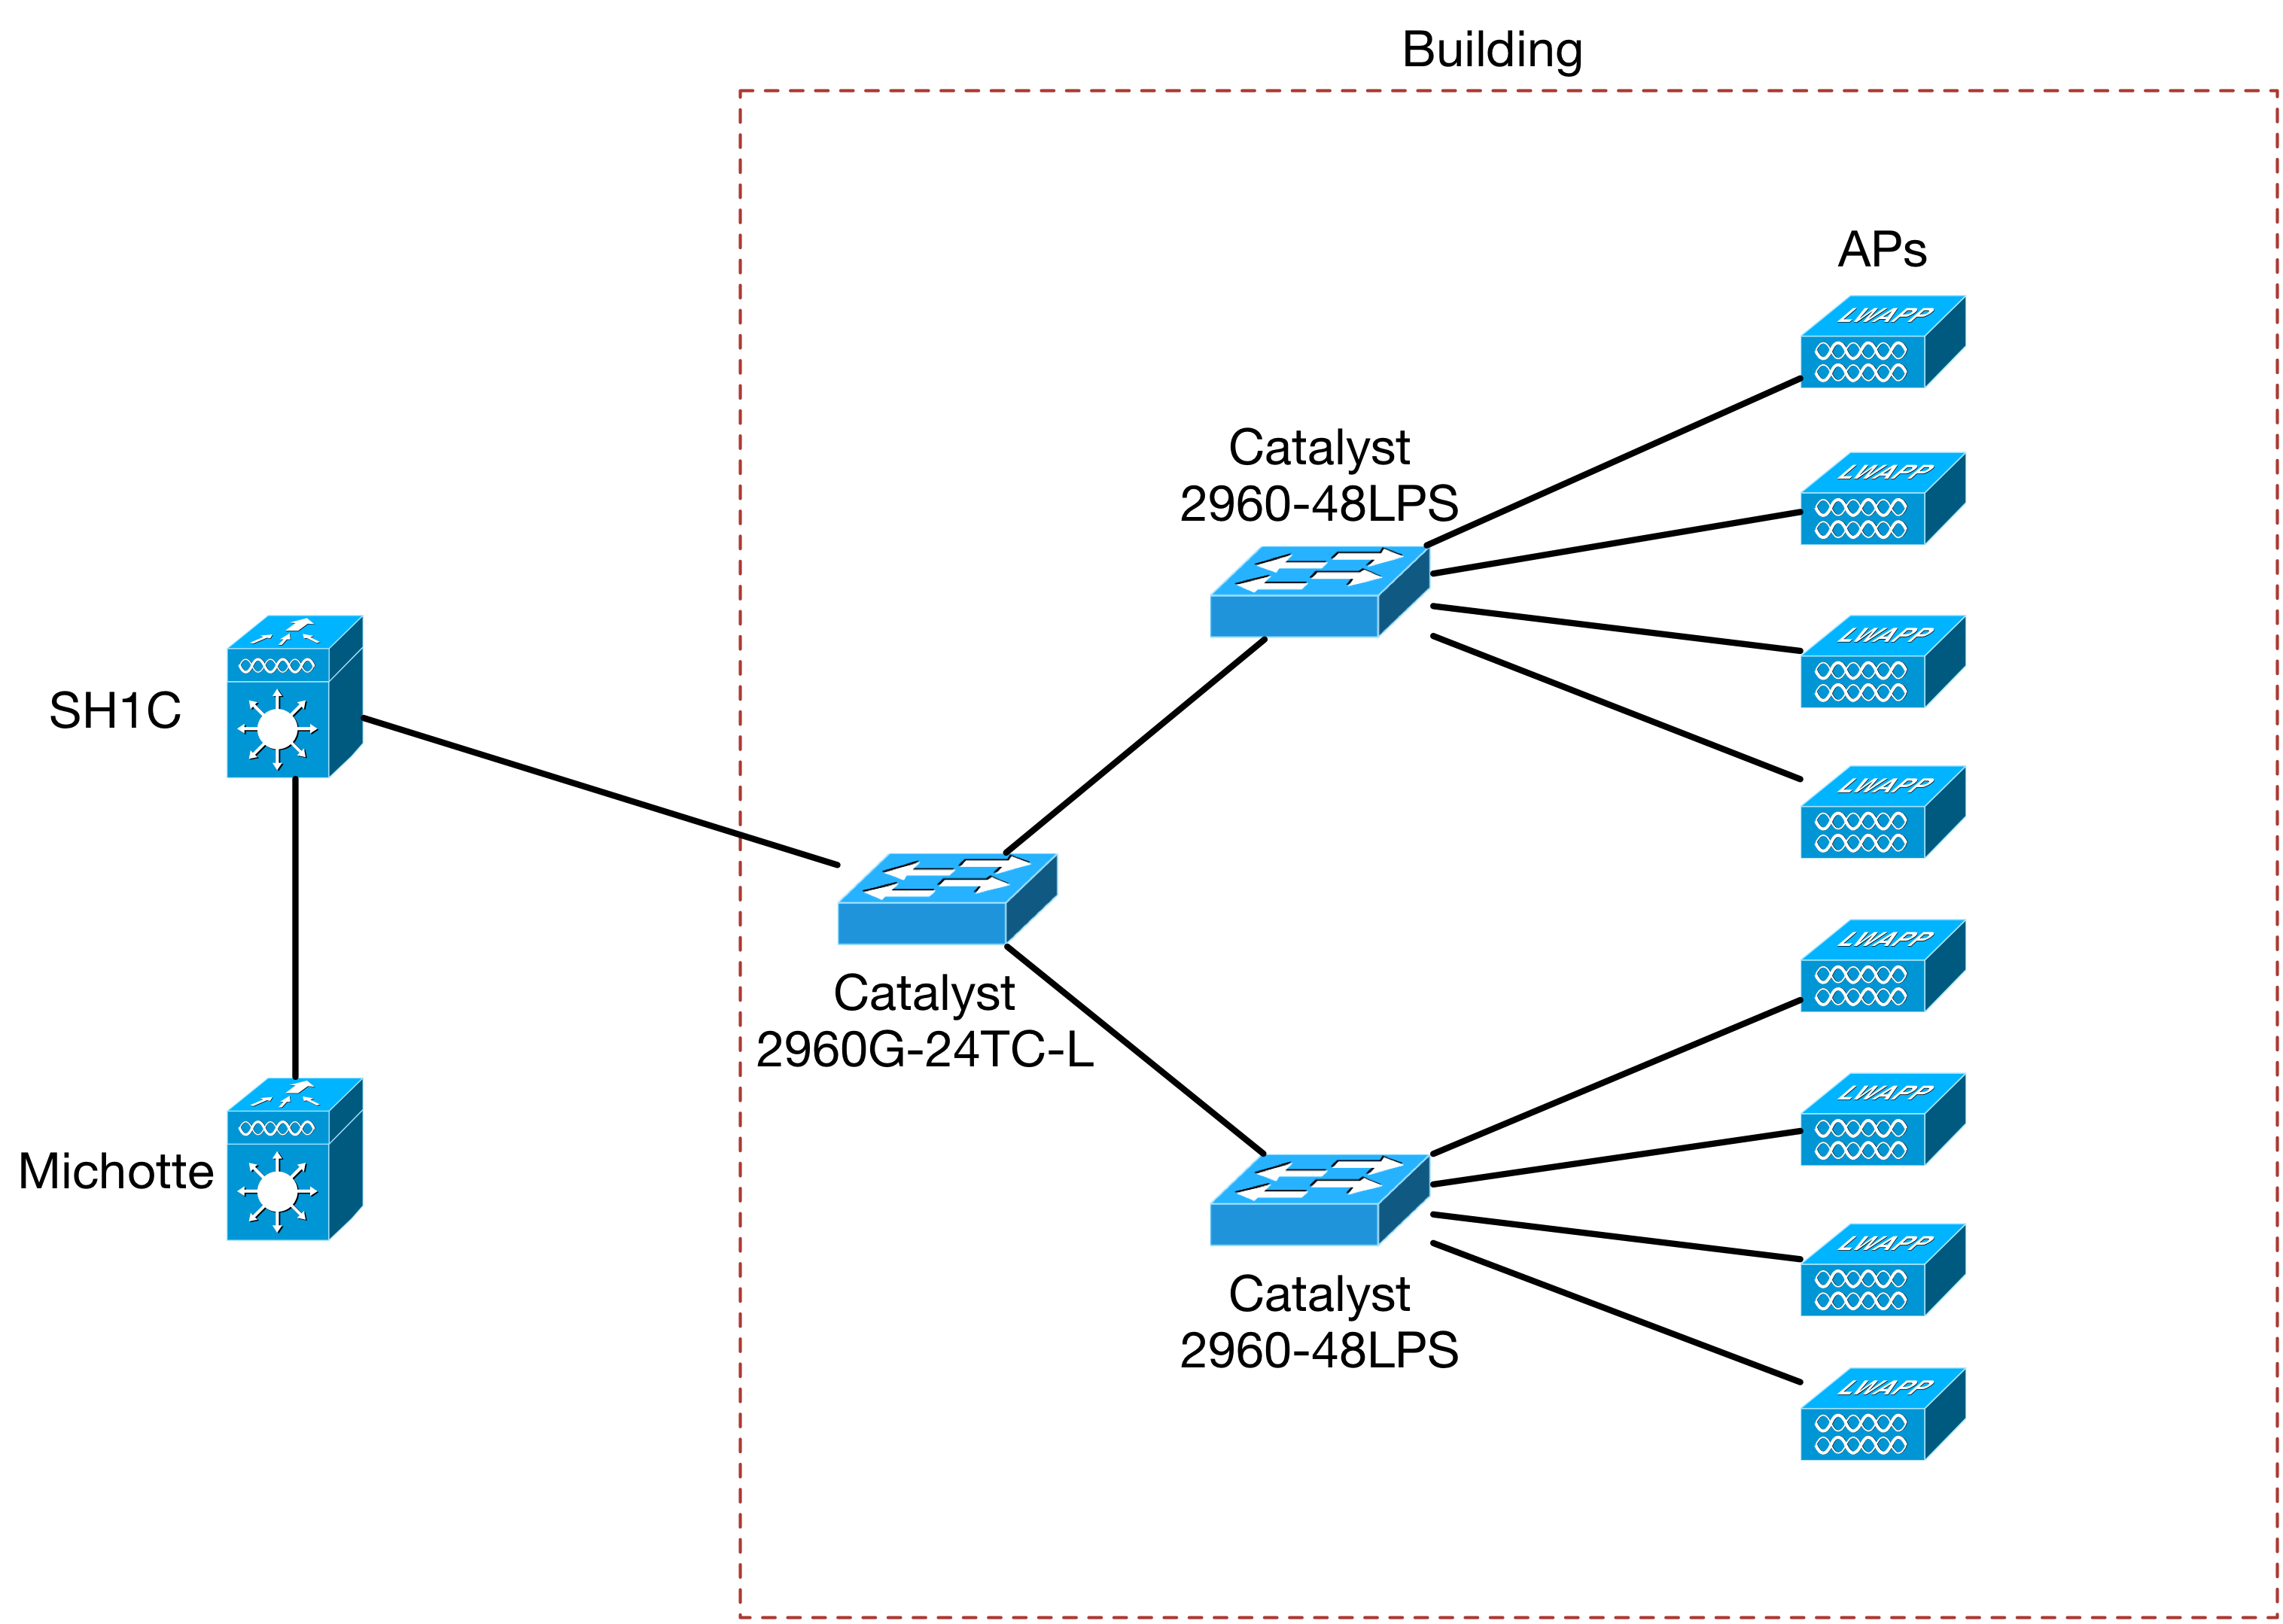
\includegraphics[width=1\linewidth]{Pictures/chapter2/building.png}
	\caption{Building infrastructure and network connection}
\end{figure}







 
% Chapter Template

\chapter{Network Components and Protocols} % Main chapter title

\label{Chapter3} % Change X to a consecutive number; for referencing this chapter elsewhere, use \ref{ChapterX}

\lhead{Chapter 3. \emph{Network Components and Protocols}} % Change X to a consecutive number; this is for the header on each page - perhaps a shortened title

%----------------------------------------------------------------------------------------
%	SECTION 1
%----------------------------------------------------------------------------------------
The purpose of this chapter is to present briefly the protocol or concepts that could be used throughout this paper.
\section{EAP}
The Extensible Authentication Protocol is a flexible authentication framework defined on the RFC3748 \cite{rfc3748}. EAP was designed to work without the IP protocol and provides support only for the transport of authentication protocols. The idea behind EAP was to creates a framework that supports several authentication methods and to separates the ahtentication methods from the transport.

\section{802.1X}
It's a IEEE standard that provides an authentication mechanism to devices on LAN or WLAN. Before explaining the standard, we will define the three parties involved.
\begin{itemize}
	\item[-]\texttt{Supplicant}: The client device that wants to connect to the network.
	\item[-]\texttt{Authentication Server}: The server that validates the credentials of the supplicants and determines the rights of the user.
	\item[-]\texttt{Authenticator}: A network device like a switch or an access point that is between the supplicant and the authentication server.
\end{itemize} 
802.1X is a port-based authentication protocol. Once a client connects to a publicly accessible port, the authenticator allows only the EAP traffic through that port. EAP is used to authenticate the supplicant and if the authentication server grants the authorization to the supplicant, it can have access to the other services.
Each port have two state:
\begin{itemize}
\item \texttt{Authorized}: In this state, the supplicant is authenticated and have access to all its services.
\item \texttt{Unauthorized}: The supplicant is not authorized and can only exchange EAP traffic with the authenticator.
\end{itemize}


\section{RADIUS}


\section{WiSM}


\section{SNMP}

The Simple Network Management Protocol is an application layer protocol that facilitates the exchange of management information between network devices \cite{snmp}. It is part of the TCP/IP protocol suite and it is mainly used by network administrators to get information about devices on the network and the network performances. These information help the administrators to resolve problems on the network or simply to manage it.
A SNMP network has three main components:

\begin{itemize}
	\item \texttt{Network-management system (NMS)}: A NMS is the main component of an SNMP-managed network. It is the management entity that controls the managed devices. It uses the SNMP protocol and can interact with the managed devices to get information using special commands and messages.
	
	\item \texttt{Managed devices}: It is a network device that contains an SNMP agent. They collect and store information to make them available for the network-management systems. Those devices can be routers, servers, switches,etc. They also run the SNMP protocols to be able to respond to the requests made by the NMS.
	
	\item \texttt{Agents}: An agent is the thinking part of a managed device. It is a software module that understands the management information and translates them into a SNMP compatible form.
\end{itemize}

\begin{figure}[H]
\centering
	\includegraphics[width=.7\linewidth]{Pictures/Chapter3/snmp.png}
	\caption{A typical SNMP managed network}
\end{figure}

All the network objects are described and organized hierarchically in a Management Information Base (MIB). There are MIBs for each set of related network entites that can be managed. These MIBs are accessed using a network-management protocol such as SNMP.


% Chapter Template
\chapter{Monitoring Tool - Implementation and Deployment} % Main chapter title

\label{Chapter4} % Change X to a consecutive number; for referencing this chapter elsewhere, use \ref{ChapterX}

\lhead{Chapter 4. \emph{Monitoring Tool - Part 2}} 

\section{NetwObserver}
The first step in the development was to select the technologies adapted to the problem. As we had a lot of log to parse, we have started the implementation using Python. Python has a strong integration of the strings and lists. It's quite easy to generate a parser of logs and keeping the code neat thanks to its very simple syntax.
As more feature were added, we need to structure the system in a way that make it easily accessible. It's a monitoring tools and it has to be accessible from everywhere and easy to use. So, we decided to implemented it as a web application. This application would be usable from every computer without any installation and the network administrators could manage and maintain it directly on the server. An update would be accessible directly for every users.

\subsection{Django: A High-Level Python Web Framework}
As presented by its developers, Django is a "web framework for perfectionist with deadlines"\footnote{\url{https://www.djangoproject.com/}}. Django allow to achieve a modular structure quite easily and provide all the developers need to add new components in the application. A Django application is composed of several modules that exists independently and interact with each other through the database.
Moreover, Django adhere to the DRY\footnote{\url{http://c2.com/cgi/wiki?DontRepeatYourself}} principle.
\begin{description}
  \item[Don't Repeat Yourself] \hfill \\
  Every piece of knowledge must have a single, unambiguous, authoritative representation within a system.
\end{description}
When we use this framework, we focus on writing and defining each element one time on the right place. Maintainability is another important component of our system. Having duplication all over the code make it difficult to maintain and to keep coherent.
Django used a variation of the Model-View-Controller model called \emph{Model-View-Template}\cite{mvt}. The main difference is that Django is not about states. Browser don't evolve from one state to another, every request are done from scratch. In MVC, Controller update the View and the Model accordingly to the events. That's not the case here because each time something is modified (e.g a new insertion in the database) we start from the beginning. It's not a defect, it's how HTTP work.

\begin{description}
\item[Model] \hfill \\
The first element that composed the application are the entities manipulated by the application. A model is a representation of an element of the domain. Each model encapsulates all the data and information required to understand it.
\item[View] \hfill \\
The main task of the views is to handle the HTTP requests. It receives a HTTP request and returns a HTTP response.
\item[Template] \hfill \\
It represents the HTTP response. It provide a generic answer and the View fulfil the missing parts (most of the time by interrogating the database).
\end{description}

Like most of the modern web frameworks, Django is built using the \emph{Object-relational mapping} technique. The purpose is to make a bridge between the object manipulated by Python and the database entries. The architecture respects an \emph{Active-record pattern} that tied each object to a row in the database. It allow to focus on the logic of the application and to code easier. We can do more with less code. The main drawback of such pattern, it's that developers tend to forget the database behind it. Even if Django is optimised to translate object in database entity (and in the other way around), it important to design the model by thinking about the database hidden behind. Every access is translated by Django but poor request or weak design could lead to really poor performance.

\subsection{MySql}
Even if most of the time we don't make direct transaction with the database, it's important to chose the right DBMS\footnote{Database Management System}. At the beginning, the capacity of the application were quite limited and we used SqLite\footnote{\url{https://sqlite.org/}}. SqLite has the particularity to not use a client-server model. It is directly managed inside the application and it is the one used by default in Django. It fits really well to small applications because all actions are internally handled and it doesn't require to install an external DBMS to handle the transactions. But quickly, we reach the limits of SqLite and we chose to migrate to MySql. NetwObserver generates several threads and make a lot of concurrent accesses to the database. Such utilization is not adapted to SqLite and made the application unstable. The main issue was that, while the application is gathering its data, it needs to still be available to the users. SqLite have some difficulties to handle insertion of a lot of new entries while getting concurrent requests from the users.

\subsection{Gatherer}
The main difficulty was to correctly gather the source of information available. For each of them, we had to implement a module to make the interface between the sources and the database. They were quite heterogeneous and the implementation required a deep understanding of them.
\subsubsection{Logs Parser}
The first source we have processed were the log files. There are three generators of log file on the network: the controller, the DHCP and the Radius. Actually, there already is a software that gathers the log files and centralized them. The tool is called Octopussy\footnote{http://www.octopussy.pm/} and is a log management solution. It allows the administrators to display the log and access them by specifying criteria like date, source or the gravity of the log. Our \emph{log} module does basically the same thing but with a deeper analysis and understanding of the content of the logs. 
\paragraph{DHCP}
The DHCP generates a log for each step of the allocation of an IP address and of course when an error occurred. Typical logs look like this:
\begin{lstlisting}[frame=single,breaklines=true,caption={DHCP logs}]
2013-10-21T17:26:00.113154+02:00 dhcp-1 dhcpd: DHCPREQUEST for 192.168.32.43 from cc:fe:3c:26:5c:3f via 192.168.35.253
2013-10-21T17:26:00.113239+02:00 dhcp-1 dhcpd: DHCPACK on 192.168.32.43 to cc:fe:3c:26:5c:3f via 192.168.35.253
2013-10-21T17:26:00.196242+02:00 dhcp-1 dhcpd: DHCPDISCOVER from 50:a4:c8:6b:48:c7 via 130.104.175.250: load balance to peer dhcp1-dhcp2
\end{lstlisting}
When the application can understand each part of the message, it allows to make more powerful links between them. If we correctly analyse each messages, we can tell, for example, which \emph{dhcpAck} correspond to a \emph{dhcpRequest}. That's a weakness of Octopussy. It can tell you what log are important and filter them but it doesn't make analysis based on the protocol. DHCP defined a succession of actions and being able to trace them make the application capable of detecting more subtle errors. Concretely, the module \emph{log} decompose the message in several part and stock it in a relational database. Even if it could seem simple, having a structured representation of the log is the first step to make better analysis on them.

\paragraph{Radius}
Radius generates logs about the authentication of the users. The main information here is the \emph{login} entered and the device used for the authentication.
\begin{lstlisting}[frame=single,breaklines=true,caption={Radius logs}]
2013-10-21T17:26:00+02:00 radius1.sri.ucl.ac.be radiusd[1523]: [ID 702911 local3.notice] Login OK: [@eur.nl] (from client WiSMPythagore-B port 29 cli e4-d5-3d-89-af-51)
2013-10-21T17:26:05+02:00 radius1.sri.ucl.ac.be radiusd[17913]: [ID 702911 local4.notice] Login incorrect: [none] (from client WiSMPythagore-A port 29 cli 00-11-e1-db-fb-5d)
2013-10-21T17:26:07+02:00 radus1.sri.ucl.ac.be radiusd[1523]: [ID 702911 local3.notice] Login OK: [53764smo@eur.nl] (from client WiSMPythagore-B port 29 cli e4-d5-3d-89-af-51)
\end{lstlisting}
Which such information we can potentially tell when and where an user was. In the other hand, it could allows to detect a device that tries to connect with different logins. That could be considered as a strange behaviour and would allow to investigate. Like in other modules, it's very important to limit the feature implemented because it could cause a ethical problem. Even if we want to make the application as complete as possible, we need to precisely define what is required and how to de it. These considerations will be discuss further in the last chapter.

\paragraph{Controller}
The more rich source of logs is the \emph{controller}. With its central position in the infrastructure, it can produce the more detailed messages when an error occurred. As the controller is made by \emph{Cisco}, the meaning of the messages can easily be found on the manufacturer website\cite{syslogCisco}.
\begin{lstlisting}[frame=single,breaklines=true,caption={Controller logs}]
2013-10-21T17:26:00.123235+02:00 192.168.251.178 WiSMPythagore-B: *spamReceiveTask: Oct 21 17:26:00.080: %LWAPP-6-CAPWAP_SUPP_VER: spam_lrad.c:1835 Discarding Primary discovery request in LWAPP from AP 00:11:bc:1b:14:00 supporting CAPWAP
2013-10-21T17:26:00.618291+02:00 192.168.251.178 WiSMPythagore-B: *mmListen: Oct 21 17:26:00.575: %MM-4-PMKCACHE_DEL_FAILED: mm_listen.c:6724 Failed to delete PMK cache entry for station 00:21:6a:86:4b:84 with request from controller 192.168.251.181
2013-10-21T17:26:00.957695+02:00 192.168.251.178 WiSMPythagore-B: *Dot1x_NW_MsgTask_0: Oct 21 17:26:00.915: %APF-6-RADIUS_OVERRIDE_DISABLED: apf_ms_radius_override.c:204 Radius overrides disabled, ignoring source 2 
\end{lstlisting}
The messages generated are very well defined and explained in the related documentation. Their structure is well defined and facilitate the parsing. Each message belong to a category and has a severity level. That allows to filter the useless ones and immediately detect the most important.

\subsubsection{SNMP}
The other main source of information is the SNMP protocol install on the \emph{controller}. This mechanism delivers a lot of indicators about the current state of the network. An important characteristic is the fact that the information is not the same as the log. While the log file represent continuously the situation and its evolution, the SNMP requests delivers a snapshot of the controller. It's a fixed representation and a comparison with an older one, doesn't give any information about what happened between the two. For example, if we had 30 people connected to an \emph{access point} at a given time and 40 one hour later, we can't conclude that ten new people have connected. Maybe the thirty people left and forty new ones had connected. We highlight this because our first architecture tried to push together the information present in the logs and in the SNMP requests. It was a bad idea because the natures of the information were completely different. It resulted in an incoherent representation of the data and make the analysis wrong or completely impossible. To correct this situation, we met Bernard Lambeau and with his advices, we have completely modified our database architecture to make a strong and deliberate separation between the different kind of data.

As said before, SNMP organized the information in a tree way. The classification of the information is quite intuitive but the main difficulty comes from the size of the tree. Once the interesting part of the tree have been identified. A lot of indicators can be gathered.

\paragraph{PySNMP} PySNMP is the module that performs the \emph{SNMP} requests. It's a pure python implementation able to perform all the standard operation i.e.\  \emph{get, set and walk}.

The \emph{snmp} module is mainly a way to create an abstraction with the snmp requests. It implements several methods to gatherer the information and make the links between them. Every request is independent and the module has to be able to know which value correspond to what element. That's the signification of the \emph{index} attribute in the \emph{Device} model.

\subsubsection{Active Monitoring}
The \emph{probe} module manages the connection with the probes. When a probe want to connect to the server, it answers and performs the authentication. When the authentication succeed, the module will receive the log file generated by the probe. Finally, it will analyse it and translate it in the database.

\subsection{Analyse}


\section{Active Probe}
As explained earlier, besides the gathering of data through \texttt{SNMP} protocol or controller's logs parsing, we also have an active data gathering process. To do that, we have implemented a \texttt{C} program that runs on an \texttt{OpenWrt} router. The following subsections give, in a first part, more details about the router used during the implementation and the tests phases as well as information about the \texttt{OpenWrt} firmware we have installed on this router. In a second part, the specifications of the program installed on that router is detailled. Information about the components and features added to that program are also explained.\\


\subsection{TP-LINK Wireless Router}
The router we use for the active monitoring process is a 150Mbps Wireless N \texttt{TP-LINK TL-WR741ND} router. This router, based on \texttt{N} technology, offers a high speed WiFi performance and is compatible with \texttt{IEEE 802.11b/g/n} WiFi standards. \\
About the hardware features, this router offers five interfaces. Four 10/100Mbps LAN ports and one 10/100Mbps WAN. It also has a 5dBi detachable omni directional antenna with a Reverse Polarity SubMiniature version A (\texttt{RP-SMA}) connector.\\
Concerning the wireless itself, the \texttt{TL-WR741ND} offers several interesting features\cite{tplink}:

\begin{description}
	\item [Frequency range]: from \texttt{2.4Ghz} to \texttt{2.4835Ghz}
	\item [Signal rate]:
		\begin{itemize}
			\item \texttt{11n}: up to 150Mbps
			\item \texttt{11g}: up to 54Mbps
			\item \texttt{11b}: up to 11Mbps
		\end{itemize}
	\item [EIRP (\textit{Effective Isotropic Radiated Power})]: $<$ 20dBm 
	%Power that the transmitter appears to have if the transmitter were an isotropic radiator (if the antenna radiated equally in all directions). EIRP = transmitter power + antenna gain - cable loss
	\item [Reception sensibility]:
		\begin{itemize}
			\item 130M: -68dBm @ 10\% Packet Error Rate
			\item 108M: -68dBm @ 10\% Packet Error Rate
			\item 54M: -68dBm @ 10\% Packet Error Rate
			\item 11M: -85dBm @ 8\% Packet Error Rate
			\item 6M: -88dBm @ 10\% Packet Error Rate
			\item 1M: -90dBm @ 8\% Packet Error Rate
		\end{itemize}
	\item [Functions]: Enable/Disable Wireless radio, WDS bridge, WMM, Wireless Statistics
	\item [Security]: 64/128/152-bit \texttt{WEP} / \texttt{WPA} / \texttt{WPA2}, \texttt{WPA-PSK} / \texttt{WPA2-PSK}
\end{description}
\begin{figure}[H]
	\begin{center}
		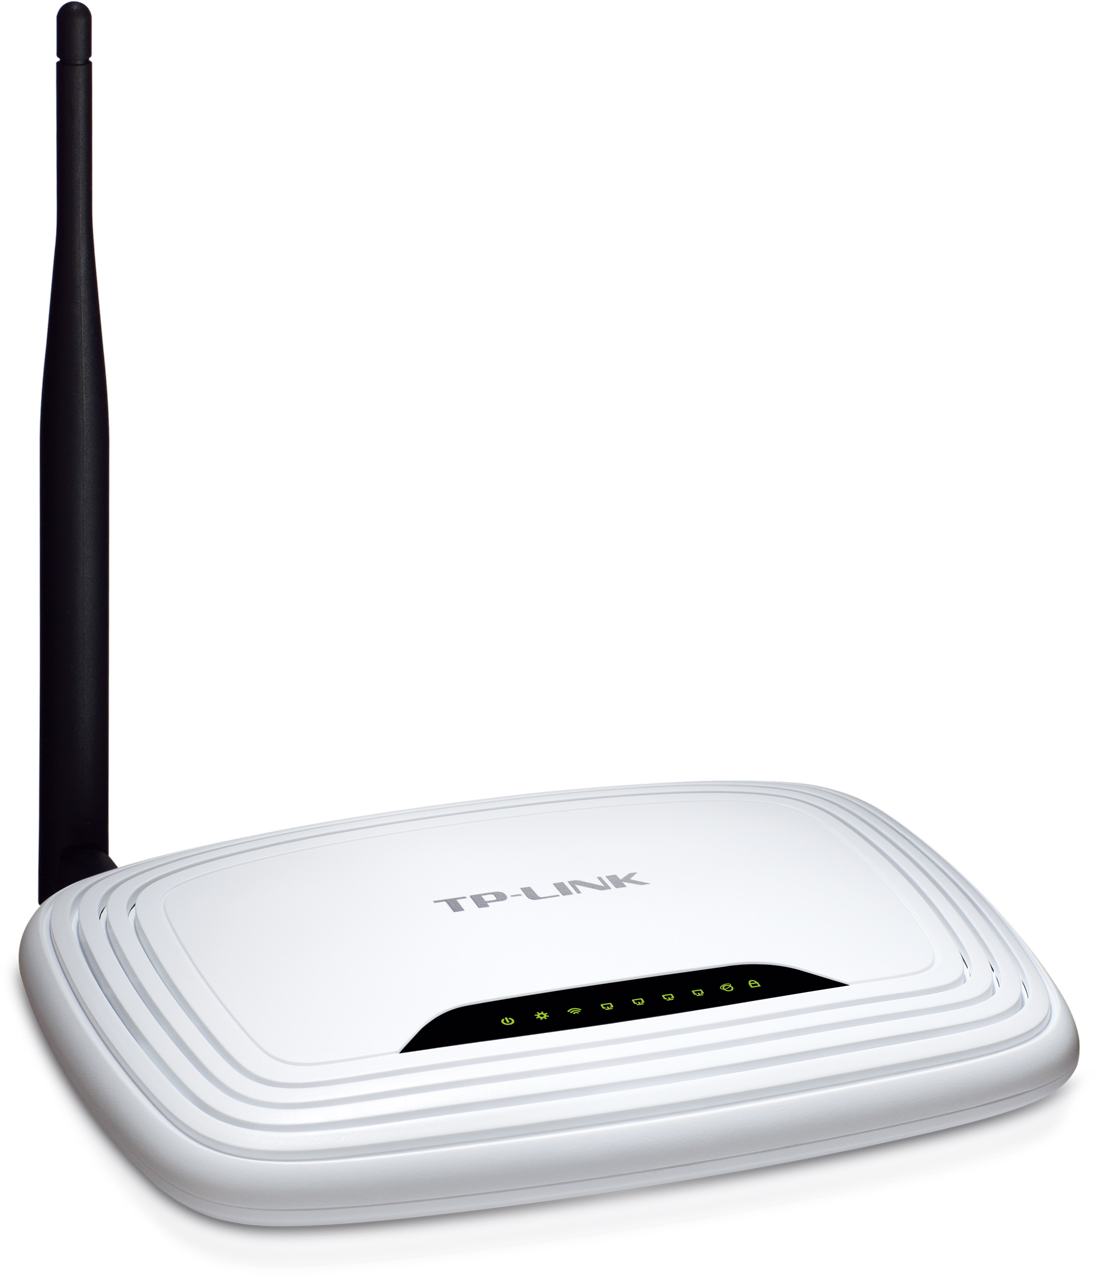
\includegraphics[width=0.26\linewidth]{Pictures/chapter4/router.jpg}
		\caption{TP-LINK TL-WR741ND}
	\end{center}
\end{figure}

To summarize, with its 150Mbps wireless data rate and its advanced WiFi security management (\texttt{WPA/WPA2} encryptions), this router provides a rather good base for our active WiFi monitoring program. But in order to be able to execute it on the probes and get results we had to change to firmware of the router to something no proprietary we can work with and we can modulate as we wish. This is why we have chosen to replace the original TP-LINK firmware installed on the router with \texttt{OpenWrt}.


\subsection{OpenWrt}
\texttt{OpenWrt}\cite{openwrt} is a highly extensible GNU/Linux distribution for embedded devices. The particularity of \texttt{OpenWrt} is that it is a full-featured, easily modifiable operation system for the routers. Indeed, it offers a fully writeable file system and a built-in package manager. Thanks to this package manager, we can install any package we want from a software repository allowing us to customize the device to suit any application. All the restrictions and configurations provided by the vendor within its own firmware installed by default on the router are therefore dropped meaning the device using this distribution can features functions such as \texttt{SSH} server, \texttt{VPN}, \texttt{BitTorrent client}, custom QoS and so on.

There are several firmwares available for \texttt{OpenWrt}. We have chosen to use the most recent one, \textit{OpenWrt 12.09 - Attitude Adjustment} for our active monitoring solution. Doing so, this ensure a reliable and up-to-date environment to deploy our application.


\subsection{Active WiFi Monitoring Solution}
Our active WiFi monitoring solution is based on a \texttt{C} program running on that \texttt{OpenWrt} router. The program uses the \texttt{wpa\_supplicant} API to be able to connect to different networks. Plus during the connection processes, a log file is created and maintained by the program to write down important information about the network's behavior. 

On this subsection we first give an overview of \texttt{wpa\_supplicant} and how we use it in our implementation. Then, we explained how our program is structured and what are the key parts that make it work and that make us able to get some insights about the networks in real time.

\subsubsection{\texttt{wpa\_supplicant}} %RSN = Robust Security Network
 As defined in \cite{wpa-supplicant}, \texttt{wpa\_supplicant} is a WPA Supplicant for Linux, BSD and Windows with support for WPA and WPA2 (\texttt{IEEE 802.11i/RSN}). Supplicant is the \texttt{IEEE 802.1X/WPA} component taht is used in the client stations. It implements key negociation with a WPA Authenticator and it can optionally control roaming and \texttt{IEEE 802.11} authentication/association of the wlan driver.

 This supplicant uses portabe \texttt{C} code and is divided into several seperate files containing independent modules besides from the core part. The core part embedded functionality for controlling the network selection, association and configuration while independent modules include code dealing with WPA (such as key handshake, pre-authentication, etc.), \texttt{EAPOL} and \texttt{EAP} state machines and methods. Also, \texttt{wpa\_supplicant} implements a control interface that we use in our program and that can control the operations of the \texttt{wpa\_supplicant} deamon.

The following figure gives an overview of all the wpa\_supplicant modules and how they interact with each other.

 \begin{figure}[H]
 	\begin{center}
		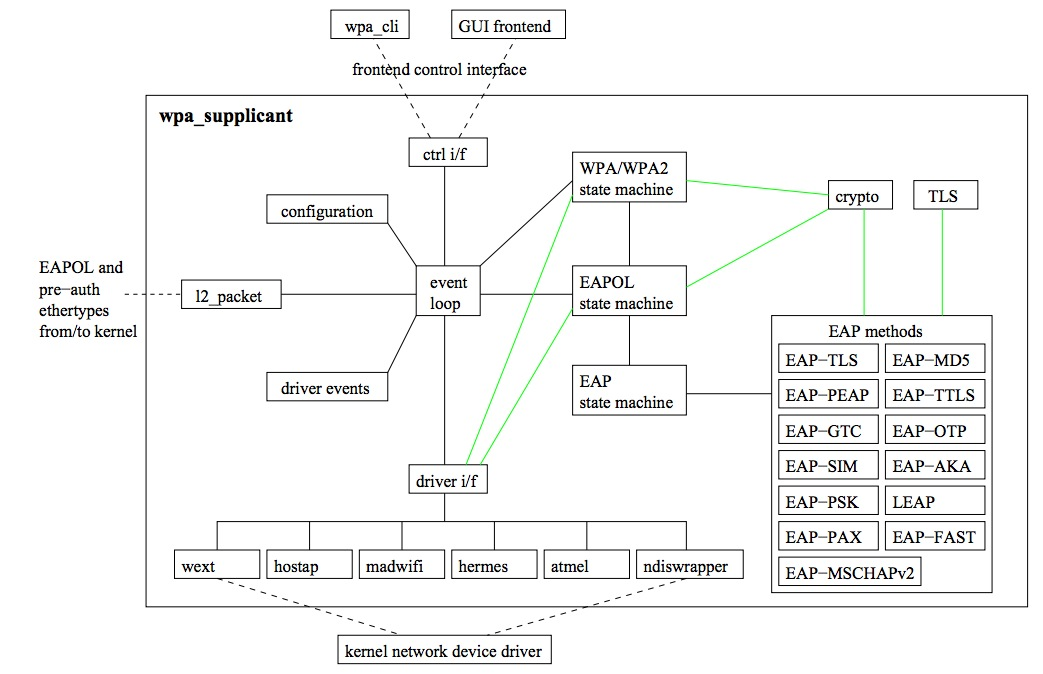
\includegraphics[width=1\linewidth]{Pictures/chapter4/wpa-supplicant-modules.jpg}
		\caption{\texttt{wpa\_supplicant} modules}
	\end{center}
\end{figure}

Within \texttt{wpa\_supplicant} there is a small \texttt{C} file, \texttt{wpa\_ctrl.c} that provides several functions to facilitate the use of that control interface. We have linked this file into program to be able to use that library of functions that can interact and communicate with \texttt{wpa\_supplicant}. Once that file is linked into the program, we can open a connection to the control interface with the \texttt{wpa\_ctrl\_open()} function and we can start sending commands to \texttt{wpa\_supplicant} with the function \texttt{wpa\_ctrl\_request()}. In order to be able to receive messages from the daemon, our program also needs to attach to the control interface using \texttt{wpa\_ctrl\_attach()}.

Several commands can be specified and sent to the \texttt{wpa\_supplicant} daemon but we only use a small selection of them, most of them being unrelated with our object of study. Here is the list of the commands used in our program and their meaning:
\begin{itemize}
	\item[-] \texttt{SCAN}: This command request the daemon to perform a new BSS scan.

	\item[-] \texttt{SCAN\_RESULTS}: This is used to get the latest scan results. Those results embed details about the bssid, the frequency, the signal level, the flags and the ssid of each network scanned. The message returned has the same syntax as in the following example representing one entry for each one of the networks of the UCL.\\

\begin{lstlisting}[frame=single,breaklines=true,caption={Scan results message exemple}]
bssid / frequency / signal level / flags / ssid
68:86:a7:30:a0:a2	2437	-56	[WPA-PSK-CCMP]	eduroam
00:1e:bd:65:34:73	2462	-55	[WPA-PSK-CCMP]	visiteurs.UCLouvain
00:1e:bd:65:34:71 	2462	-56	[WPA-PSK-CCMP]	student.UCLouvain
68:86:a7:30:a0:a0 	2437	-55	[WPA-PSK-CCMP]	UCLouvain
68:86:a7:30:a0:a4 	2437	-57	[WPA-PSK-CCMP]	UCLouvain-prive
\end{lstlisting}

	\item[-] \texttt{ADD\_NETWORK}: This commands adds a new network with empty configuration. This added network is disabled at first and can be configured afterwards. The commands returns a message containing the id of the new network or \texttt{FAIL} on failure. In our case, the program adds 5 networks at boot for the 5 networks present within the university's campus.

	\item[-] \texttt{SET\_NETWORK <network id> <variable> <value>}: Once the networks had been added with the previous command, we can configure them using this particular command. The \textit{variable} of the command uses the same variables and data formats as the standard \texttt{wpa\_supplicant} configuration file. For example, here are the different \texttt{SET\_NETWORK} commands used to configure the \texttt{student.UCLouvain} (with ID=1 for example) that we use in the program.\\

\begin{lstlisting}[frame=single,breaklines=true,caption={Configuration of the \texttt{student.UCLouvain} network}]
SET_NETWORK 1 ssid "student.UCLouvain"
SET_NETWORK 1 key_mgmt WPA-EAP
SET_NETWORK 1 eap TTLS
SET_NETWORK 1 identity "login@wifi.uclouvain.be"
SET_NETWORK 1 password "password"
SET_NETWORK 1 ca_cert "etc/wpa_supplicant/chain-radius.pem"
SET_NETWORK 1 pahse2 "auth=PAP"
\end{lstlisting}

	\item[-] \texttt{SELECT\_NETWORK <network id>}: This command asks the \texttt{wpa\_supplicant} daemon to select a special network specifying its ID. When the network is selected, all the others are disabled.

	\item[-] \texttt{DISCONNECT}: Special command to disconnect from the current network.
\end{itemize}

Thanks to does commands our program can to control the \texttt{wpa\_supplicant} daemon and is thus able to simulate a typical user's behavior connection to the networks. More information about \texttt{wpa\_supplicant} can be found inside the developer's guide\cite{wpa-supplicant-devel}.


\subsubsection{\texttt{wifi\_minitoring.c}}
In this section we describe the implementation details of our active monitoring program and how it gathers data about the current state of the networks.

The first thing the program does at boot is to start \texttt{wpa\_supplicant}. We have created an empty configuration file for the supplicant in order to launch it without starting a connection to a special network defined in that file. The supplicant uses the driver \texttt{nl80211} which is the current standard (\texttt{wext} being deprecated) and uses the \texttt{wlan0} interface.
Once the supplicant is started we open a connection with the control interface using \texttt{wpa\_ctrl\_attach(/tmp/run/wpa\_supplicant/wlan0)} (where the parameter is the path for UNIX domain sockets). That function returns a pointer to the abstract control interface data and is stored inside an internal \texttt{wpa\_ctrl} structure.






\section{Communication between Server and Probes}
The probes and the server have to exchange information. As we wanted to create a modular tool, we have chosen to encrypt all the data sent between the server and the probes. If the active monitoring device capture sensible contents, there must be no security vulnerabilities like \emph{eavesdropping} or \emph{man-in-the-middle attack}.
The first constraint that appeared was the weak computation power of the probes. In consequence, we had to keep the encryption as easy to perform as possible. So, we have looked into \emph{symmetric cryptographic} techniques. But in the other hand, as we have several probes, it could be difficult to manage and exchange the keys unlike in asymmetric cryptography. Our choice was to take the best of both worlds and implement a protocol using hybrid encryption.
In definitive, we used RSA and AES encryption together.
\subsection{RSA}
RSA\footnote{\url{http://www.google.com/patents/US4405829}} is one of the most used \emph{public-key cryptosystem}. Its name comes from its three designers: Ron Rivest, Adi Shamir, and Leonard Adleman. The algorithm involves two key: a \emph{public key} known by everybody and a \emph{private key} kept secret. The safety ensured by the technique comes from the difficulty of the factoring problem (factoring the product of two large prime numbers).
The main advantage against symmetric cryptography is that the public key used for the encryption can be known by everybody and so make the problem of key exchange a lot easier. To make the explication clearer we will present a simple example occurring between Alice and Bob.
\begin{enumerate}
\item Alice give her public key to Bob.
\item Bob wants to transmit a encrypted message to Alice. He uses the Alice's \emph{public key} to encrypt the message.
\item Bob sends his message to Alice. Even if people intercept the transmission and have the public key, they couldn't decrypt it.
\item Alice receives the message and decrypt it with her private key which she have kept secret.
\end{enumerate}
The key is 2048 bits long and each entity has its own pair of keys (i.e. the server and each probe). The server will known the authorized probes by having their private keys and will use them to encrypt the AES key (see below).
The main drawback of such encryption is that the computations are quite heavy to perform. Which is against our previous requirements. That's why we only use it to encrypt and exchange a symmetric key that will be used for the exchange of data.
\subsection{AES}
The symmetric algorithm used is AES which stands for Advanced Encryption Standard. We chose a size of 256 bits for the keys which is quite correct for our utilization. The idea is to permute the bits of the message using the key. The operations performed are lighter than the ones used by RSA and so make it more adapted to be used on the probes.

\subsection{Transaction Protocol}
To be correct, the exchanges between the probes and the server requires a protocol well defined and respected by the two parts. 



As already said, the server knows the public key of every probe in advance. 



\subsection{OpenSSL}

\subsection{PyCrypto}

\section{Deployment}
For the deployement of our system, we had a dedicated machine to host our data. This system was quite limited to be able to efficiently serve the requests. The server have a hard drive of about 300GB which is quite enough to stock the information gathered by NetwObserver during the test phase. In the other hand, the memory available was only of 1GB which is not enough to ensure a efficient handling of the users requests.

\subsection{Apache 2}
As the interface of the system is composed of Web pages, the HTTP requests are handle by Apache2. As the most used server, we had a lot of documentation available. That was the main reason of our choice. Moreover, we thought that a first experience in server configuration would be an interesting experience for any computer science students.

\subsection{Module WSGI}
This Apache module is able to interpret some python code. As said before, we choose Django as framework and in consequence executing python code is an important requirement. Something to note about the installation is that the code is written in \emph{Python3.3} and not in the version 2. That's force to be carreful during the installation as the default python interpreter in most system is the 2.6. In definitive, we have to compile the module WSGI with the specification of the right interpreter.

\subsection{Celery}
Celery\footnote{http://www.celeryproject.org/} is a distributed task queue. It allows to create asynchronous jobs handled by several workers. Concretely, a worker is a external thread that receives tasks to accomplished. the main drawback of \emph{Apache} is that it's quite complicated to generate and manage daemon running in background constantly or at given intervals. As a turn-around, we have connected our system to Celery. It helps us to manage more efficiently the concurrent elements of the application. Our server has a small memory and a poor computation power and in consequence we must manage and organise the utilization of those resources. This module has two main component: the workers and the scheduler.

\subsubsection*{The workers}
In Celery, we can define the number of workers working on the task send to the queue. By adapting this number, we can tune the allocation of the processor. For example, when we lunch a set of \emph{SNMP} requests, it can require a large part of the available resources. Each of these set of requests are lunch at different intervals and can sometime overlap. When that situation occurred, the server can experience heavy computation requirements and have trouble to handle the requests generated by the users. That's why we define a fixed number of workers and each tasks wait in a queue till a slot are available. The main drawback of such architecture is that the the precise moment when the jobs is effectively done is undetermined. Even if it can be really annoying in certain context, it is not the case in our system. Either we have a daemon that run permanently as the one handling the communication with the probes or the task have to gather some data at some interval. This last category have not precise time requirement and even if they happen dozens of minutes later, it's not a really issue here.

\subsubsection*{The Scheduler}
The scheduler in Celery is called \emph{beat} and its only responsibility is to send the \emph{periodic tasks} to the workers. We have given it the path of the application i which we have define the task and the related interval. \emph{Celery beat} gatherer them and fire the task accordingly. The main warning about the scheduler is the fact that it lunch the task \textbf{exactly} at each interval. If we imagine a task that take between 4 and 5 minutes to be perform and that the interval is of 10 minutes, there can be moments where two instances of that tasks overlap. Effectively, if all the workers are occupied and the first instance only start after 8 minutes of waiting, the second task will start two minutes later while the first one is still running. Here again, such consideration have been taken care of and the data are store with a time stamp or linked to en entity having one. The data gatherer can be completely order and even if such condition occurred, the result would be only a lack of data during an interval and more during the next one. As the intervals vary from 20 minutes to 2 hours while the results are analyse throught several day of data, the impact is quite reduced. 

\section{Extensions and Portability}
 
% Chapter Template

\chapter{Analysis and Results - Passive Monitoring} % Main chapter title

\label{Chapter5} % Change X to a consecutive number; for referencing this chapter elsewhere, use \ref{ChapterX}

\lhead{Chapter 5. \emph{Analysis and Results - Passive Monitoring}} % Change X to a consecutive number; this is for the header on each page - perhaps a shortened title

\section{Analysis}
The final purpose of our system is to provide analysis about the main issues we have encountered on the wireless infrastructure. The way we process here is quite simple:

\begin{enumerate}
\item Aggregate related information
\item Spot anomalies
\item Try to understand the causes
\end{enumerate}

Like in any other system, we had to define domains on which the monitoring tool will be able to work. As a reminder, one of the first steps of this thesis was to determine what are, or could be, the main issues on the UCL's wireless network. This is typically during this step that we will use those results. Each of these problems will be represented by a domain in which we will define what the relevant data are, how they can help us, and how to correctly react after having analysed them. 

The purpose of this chapter is to present these domains and the methodology we used to analyse them since they all have their particular needs and their related techniques of analysis.

\section{WiFi}

\subsection{Users}
This first section of the application offers some aggregated statistics about the users of the wireless network. The main objective is to get some analysis about the actual utilization of the wireless infrastructure. It can be seen like a set of indicators that help the administrators get a global and live overview of the network. 

\subsubsection*{WiFi Protocol}

The following graph displays the repartition of users among the available \texttt{IEEE 802.11} standards (i.e. \texttt{802.11a, b, g, n}). 

\begin{figure}[H]
	\centering
   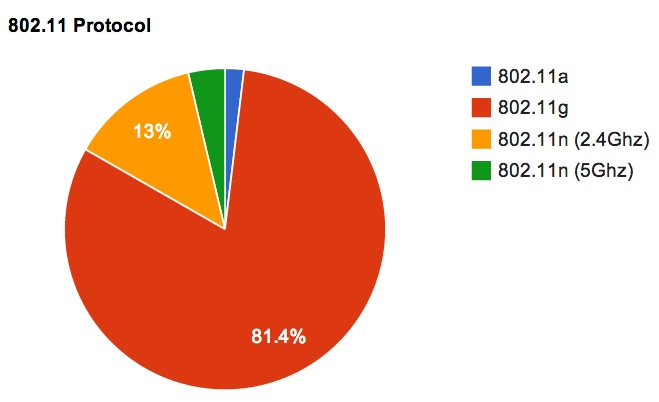
\includegraphics[width=0.6\textwidth]{Pictures/chapter5/ip-proto.jpg}
   \caption{Repartition of users among the \texttt{IEEE 802.11} standards.}
\end{figure} 

The reason for this analysis came because of an earlier policy enforced on the UCL's network that forbids the use of the \texttt{802.11b} protocol. Indeed, users connecting to the network with such low bandwidth standard force the access points to transmit for a longer time and can, by consequence, prevent the other users from achieving high receiving speeds. This analysis was designed to help the administrators have future information in the same domain. By profiling the habits of the users, we can define the impact of such decision on the wireless protocols. Indeed, since the quality of the service is one of the main concerns, deactivating the utilization of a standard used by most of the devices could have heavy consequences.

The statistics are based, by default, on the connection establishments made during the last three months. This to ensure that devices no longer connected to the network do not affect the results, and to keep the analysis as up-to-date as possible.

\paragraph*{Sources} The data used come from \texttt{SNMP} requests. During each cycle we gather information about all the devices associated with the access points. All the descriptions and details about the \texttt{OID} come from the \texttt{Cisco OID Browser}\footnote{http://tools.cisco.com/Support/SNMP/do/BrowseOID.do}.

\noindent
\begin{tabular}{|r l|}
\hline 
\textbf{Object} & \texttt{bsnMobileStationProtocol} \\
\textbf{Description} & \parbox{11cm}{The \texttt{802.11} protocol type of the client. The protocol is mobile when this client detail is seen on the anchor i.e. it is mobility status is anchor.} \\
\textbf{OID} & 1.3.6.1.4.1.14179.2.1.4.1.25 \\
\textbf{MIB} & AIRESPACE-WIRELESS-MIB \\
\hline
\end{tabular}

\subsubsection*{SSID Utilization}
Here, we compute the number of users by \texttt{SSID}. As before, the goal is to provide a complete profile of the network's users to the administrators. Such measurement can help them to adjust the policies related to each \texttt{VLAN} and defining the load of each one of them. It could help to diagnose a useless \texttt{VLAN} or in the opposite, it could allow to detect an overloaded one that might be caused by an improper utilization of the network. The supposed and the actual utilization of the network can be really different and such indicators can help the administrators to adjust the \texttt{VLAN} configurations. Here is the representation of the \texttt{VLANs} utilization we computed during our deployment phase.
\begin{figure}[H]
	\centering
   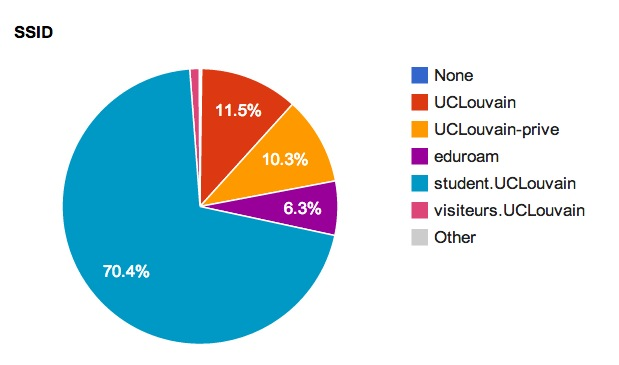
\includegraphics[width=0.7\textwidth]{Pictures/chapter5/ssid-utilization.jpg}
   \caption{\texttt{SSID} utilization}
\end{figure} 

\paragraph*{Sources} As before, we mainly aggregate the data available on the controller.

\begin{tabular}{|r l|}
\hline
\textbf{Object} & \texttt{bsnMobileStationSsid} \\
\textbf{Description} & \parbox{11cm}{The SSID Advertised by Mobile Station.} \\
\textbf{OID} & 1.3.6.1.4.1.14179.2.1.4.1.7 \\
\textbf{MIB} & AIRESPACE-WIRELESS-MIB \\
\hline
\end{tabular}

\subsection{Access Points}
This section regroups several analysis related to the access points. In a network with several hundreds of access points, it can be difficult to diagnose and monitor each one of them. By centralizing and aggregating the data, we help the network managers to save time by automatizing lots of computations. In this part of the application, we have access to the monitoring information of each access point currently associated with the controller.

\subsubsection*{Load}
A fundamental piece of information related to an access point is its load. We monitor each spot continuously and record its state several times per hour. By analyzing those data, we are able to plot graphs representing the load of the access point throughout the days. To do that, we need two information: the \textit{quantity} of data transiting on the link and the \textit{maximum speed} of that link. Concretely, each \texttt{AP} owns two byte counters that are incremented each time a byte is received or sent. The other information required is the speed of the link connecting the AP to the network infrastructure (this information on itself can be useful to diagnose bandwidth issues).

\paragraph*{Links} In a large-scale network, it can be difficult to keep track of which links are up-to-date and which ones were updated yet. By collecting these data, we were able to find that two access points were still connected with a \texttt{10Mbps} link. For this particular case, the cause was that those two devices were not managed by the \texttt{SGSI} and in consequence were not upgraded with the others. Those APs are located in the \texttt{Stevin} building.
This is an example that even such simple collected data can help diagnose some inconsistencies in the network.

\begin{figure}[H]
   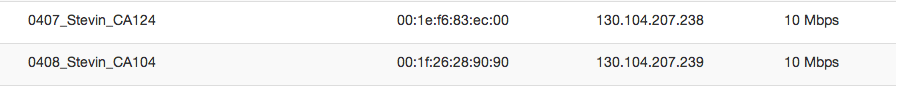
\includegraphics[width=\textwidth]{Pictures/chapter5/slowLinks.png}
   \caption{Example of 10Mbits Links (26/06/2014)}
\end{figure}

\paragraph*{Pattern of Utilization} By taking a look at the results, we can see during which periods of time the access points are the most active. In the example below, we have chosen an access point located in the \texttt{Leclercq} building and displayed the results of several days of monitoring. As expected, almost no activity is detected during the night. It really starts around 9 am. 

\begin{figure}[H]
   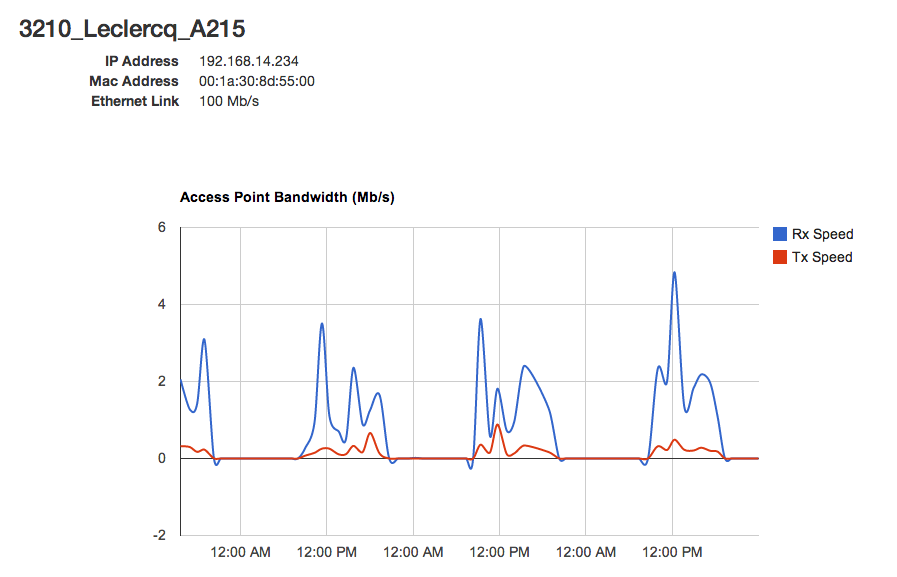
\includegraphics[width=\textwidth]{Pictures/chapter5/apLoad.png}
   \caption{Access Point Load}
\end{figure}

\paragraph*{Overloaded AP} Finally, we check the access points that have a \emph{medium utilization} superior to a specific threshold (defined by the user). We count the number of times such overload has been detected and we display the access points accordingly in a decreasing order. The result allows us to determine what are the busiest APs of the infrastructure. Here is an example of the four busiest APs of the infrastructure at the time of our deployment phase.

\begin{figure}[H]
   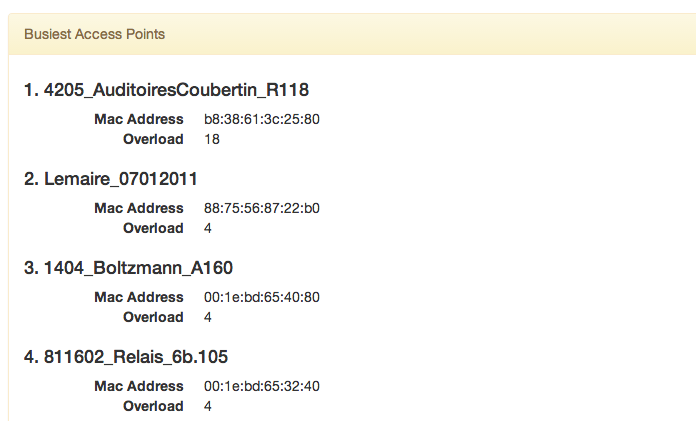
\includegraphics[width=\textwidth]{Pictures/chapter5/busiestAP.png}
   \caption{Example of busiest Access Point}
\end{figure}

\paragraph*{Sources} Here again, we use the data available on the controller. The first data collected are the byte counters of each access point.

\begin{tabular}{|r l|}
\hline
\textbf{Object} & \texttt{cLApEthernetIfRxTotalBytes} \\
\textbf{Description} & \parbox{11cm}{This object represents the total number of bytes in the error-free packets received on the interface.} \\
\textbf{OID} & 1.3.6.1.4.1.9.9.513.1.2.2.1.13 \\
\textbf{MIB} & CISCO-LWAPP-AP-MIB \\
\hline
\end{tabular}

\begin{tabular}{|r l|}
\hline
\textbf{Object} & \texttt{cLApEthernetIfTxTotalBytes} \\
\textbf{Description} & \parbox{11cm}{This object represents the total number of bytes in the error-free packets transmitted on the interface.} \\
\textbf{OID} & 1.3.6.1.4.1.9.9.513.1.2.2.1.14 \\
\textbf{MIB} & CISCO-LWAPP-AP-MIB \\
\hline
\end{tabular}

The next step is to obtain the speed of each link connected to an access point. This time again we use the \texttt{SNMP} protocol to get the information from the controller.

\begin{tabular}{|r l|}
\hline
\textbf{Object} & \texttt{cLApEthernetIfLinkSpeed} \\
\textbf{Description} & \parbox{11cm}{Speed of the interface in units of 1,000,000 bits per second.} \\
\textbf{OID} & 1.3.6.1.4.1.9.9.513.1.2.2.1.11 \\
\textbf{MIB} & CISCO-LWAPP-AP-MIB \\
\hline
\end{tabular} 

\subsubsection*{Interfaces}
Each access point has two WiFi interfaces. The first one emits at \texttt{2,4Ghz} and the second at \texttt{5Ghz}. For each interface, the controller provides a lot of information that can be used in parallel with the previous ones. The first information that we gather is the \textit{number of users} currently associated to the interface. We complete that information with the quantity of users with a poor \texttt{Signal-Noise Ratio} (SNR). This analysis allows to diagnose the efficiency of the access point. Even if it may be considered normal to have a couple of users with a poor \texttt{SNR}, if the proportion is constantly high, it can be an indicator that a additional access point might be helpful, or that the location of the AP is problematic. The problems have to be put in perspective with the \texttt{RF} environment (i.e. \texttt{Rogue Access Points} or physical walls) which is outside the scope of this monitoring system. 
Finally, we complete this analysis with a monitoring of the \emph{channel utilization}. A high utilization of the channel results in poor connection quality for the user and could indicates weak \texttt{RF} conditions.
Here is a representation of a \texttt{2.4GHz} interface with information related to the clients occupancy, the occupancy of clients with a poor \texttt{SNR} and the channel utilization. 

\begin{figure}[H]
   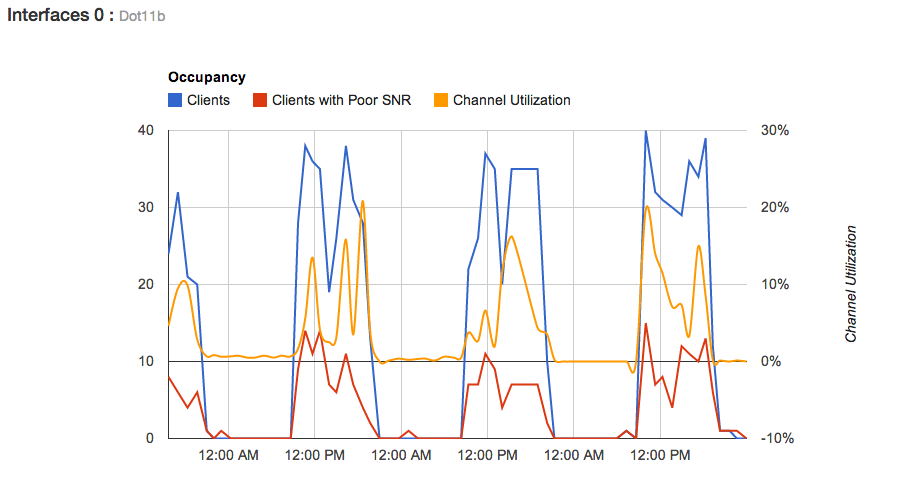
\includegraphics[width=\textwidth]{Pictures/chapter5/interfaceLoad.png}
   \caption{A 2,4GHz Interface}
\end{figure}

\paragraph*{Poor SNR} To illustrate our results, we have taken the \texttt{2,4GHz} interface of the previous access point (i.e. \texttt{3210 Leclercq A215}) during the same period of time. As we can see, the load of the access point is correlated with the number of people connected to the interface. In this situation, we observe that there is an average of one-third or one-fourth of users with a poor \texttt{SNR}. This can be related to the configuration of the building. There is a large number of walls that separate the class rooms. The last thing to consider is the definition of a \emph{poor} \texttt{SNR}. This value is completely defined by the controller. In definitive, we do not have any access nor control on that parameter. Finally, in order to understand the importance of this result, we have to be aware that if a large portion of users has a low signal, it might influence the other devices with a good one. Indeed, the access points may have to spend more time sending data to those users with a low signal and, by consequence, are unavailable for others connections.

\paragraph*{Channel Utilization} The channel is a shared resource and need to be available in order to be used. The utilization of the channel is an important monitoring indicator. It allows the network administrators to estimate the quality of the users connections. If the medium is used at more than fifty percent, latency-sensitive applications can experience some performance issues \cite{ciscoVowlan}. A continuous monitoring of that value can help to detect and diagnose such related problems. In our example, we can see that there is some maximum peaks at twenty percent of utilization which are totally acceptable. 


\paragraph*{Sources} The controller keeps entries for each interface of each access point. We gather and cross all these data to generate some entries about each \emph{access point} and all the related \emph{interfaces} that are inserted into the database.

\begin{tabular}{|r l|}
\hline
\textbf{Object} & \texttt{bsnAPIfLoadNumOfClients} \\
\textbf{Description} & \parbox{11cm}{This is the number of clients attached to this Airespace AP at the last measurement interval.} \\
\textbf{OID} & 1.3.6.1.4.1.14179.2.2.13.1.4 \\
\textbf{MIB} & AIRESPACE-WIRELESS-MIB \\
\hline
\end{tabular}

\begin{tabular}{|r l|}
\hline
\textbf{Object} & \texttt{bsnAPIfPoorSNRClients} \\
\textbf{Description} & \parbox{11cm}{This is the number of clients with poor SNR attached to this Airespace AP at the last measurement interval.} \\
\textbf{OID} & 1.3.6.1.4.1.14179.2.2.13.1.24 \\
\textbf{MIB} & AIRESPACE-WIRELESS-MIB \\
\hline
\end{tabular}

\begin{tabular}{|r l|}
\hline
\textbf{Object} & \texttt{bsnAPIfLoadChannelUtilization} \\
\textbf{Description} & \parbox{11cm}{Channel Utilization.} \\
\textbf{OID} & 1.3.6.1.4.1.14179.2.2.13.1.3 \\
\textbf{MIB} & AIRESPACE-WIRELESS-MIB \\
\hline
\end{tabular}

\subsection{Rogue Access Points}
For the \texttt{rogue access points}, we chose to group them by their estimated location. For each one of them, we know what is the closest AP that is able to detect it. Thanks to that information we can tell where those rogue access points are and we can generate aggregated information about the areas that contain the more of them. To group the rogue access points, the system uses a dictionary implemented as a \texttt{JSON} file. This file defines some \texttt{tags} and their related \emph{group}. For each rogue AP, the name of the closest access point is checked. If it contains a tag, the rogue AP is added to the related group. The rogue AP with no groups are left over. The listing gives representation of what a zone dictionary looks like. The figure below shows the number of rogue access points by area.

\begin{lstlisting}[frame=single,breaklines=true,caption={Example of a Zone Dictionary}]
{
	"Halles":"Halles",
	"Reaumur":"Sciences"
	"Croix":"Sciences"	
}
\end{lstlisting}

\begin{figure}[H]
   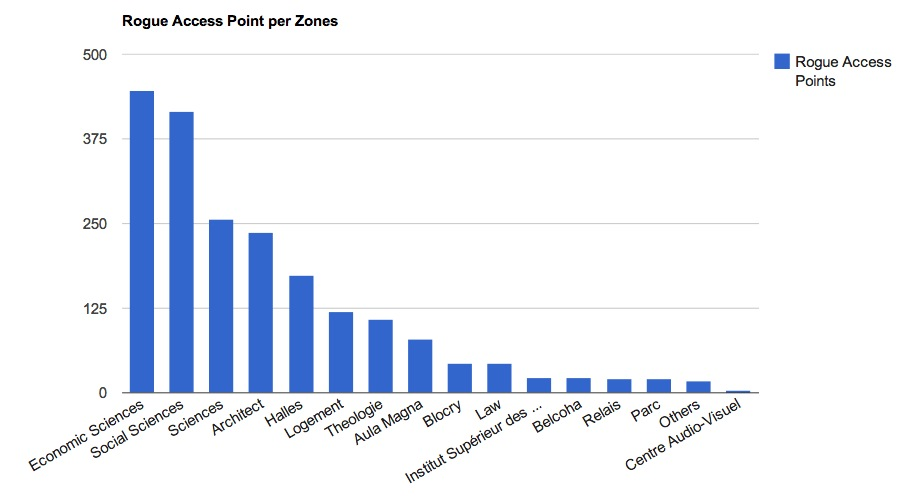
\includegraphics[width=\textwidth]{Pictures/chapter5/rogue-ap.jpg}
   \caption{Number of Rogue AP by area}
\end{figure}

\paragraph*{Sources} The sources are the access points themselves. Each one of them reports to the controller what are the rogue access points they are able to detect. The controller centralizes all those information and make them available through \texttt{SNMP}.

\begin{tabular}{|r l|}
\hline
\textbf{Object} & \texttt{bsnRogueAPDot11MacAddress} \\
\textbf{Description} & \parbox{11cm}{MAC Address of Rogue Station.} \\
\textbf{OID} & 1.3.6.1.4.1.14179.2.1.7.1.1 \\
\textbf{MIB} & AIRESPACE-WIRELESS-MIB \\
\hline
\end{tabular}

\begin{tabular}{|r l|}
\hline
\textbf{Object} & \texttt{bsnRogueAPDetectingAPMacAddress} \\
\textbf{Description} & \parbox{11cm}{MAC Address of of detecting AP which received max RSSI.} \\
\textbf{OID} & 1.3.6.1.4.1.14179.2.1.7.1.13 \\
\textbf{MIB} & AIRESPACE-WIRELESS-MIB \\
\hline
\end{tabular}



\section{Controller}
The controller logs are divided in several categories. Each one of them defines a list of logs related to that category. The main idea here is to analyse the activity of each domain of logs and try to spot irregularities. We make the hypothesis that when something goes wrong, the related category emits a larger amount of logs. By monitoring that activity, we are be able to identify in which part of the infrastructure the issue happened. More powerful analysis could be easily implemented but that would require to target some specific syslogs. That could be really useful if the administrators want to monitor specific events and detect certain patterns. But that is only relevant in order to detect very precise elements, and we have chosen to focus on a more global monitoring system.


\subsection{Components Activity}
The idea here is to have a representation of the logs generated by each component throughout the day. With such representation, we can detect some peaks of activity that could indicate an issue. Our graph displays the overall static activity but if a direct and stable access with the controller can be created in order to retrieve the logs dynamically, a representation throughout time would be possible and would be very useful in order to spot more easily the anomalies.

\begin{figure}[H]
	\centering
   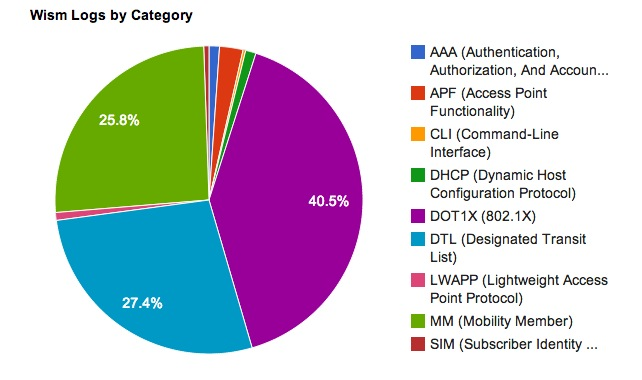
\includegraphics[width=0.74\textwidth]{Pictures/chapter5/controller.png}
   \caption{Example of Controller Activity}
\end{figure}

\section{DHCP}
These analyses aim to detect \texttt{DHCP} related issues. The allocation of IP addresses is a fundamental component in wireless networks. Being able to detect when \texttt{DHCHP} problems appears and notify them directly in our application might help making a quicker and more efficient response.

\subsection{Leases}
The main challenge with a \texttt{DHCP} server is the configuration of the \texttt{IP} address ranges. It is always difficult to determine the quantity of IP addresses the \texttt{VLANs} require. If no \texttt{IP} address is available for a user, he won't be able to access the Internet despite the fact that he has already established a connection with the AP. The main issue is that when such problems arise it can be tricky to be aware of them. Indeed, most of the time the users do not report the problem to the network administrators or if they do, their explanations of the problem are not very precise, complicating the tasks of those administrators. Being able to automatically detect the lack of \texttt{IP} addresses can thus be very time saving. Even if those information are available within the \texttt{DHCP} logs and that those servers can send warnings in case of trouble, centralizing and aggregating them with data related to all the other network components may lead to more powerful analysis.


\paragraph*{Misleading Error Messages} When we started to investigate on this issue, we tried to find what kind of logs the \texttt{DHCP} servers had generated in such circumstances. The answer is that the servers simply indicate that situation by adding \texttt{peer holds all free leases} next to the \texttt{Discover} event. So, we have searched for such messages in the log files and we have found some of them among other normal \texttt{Discover} messages. It seems odd that if no lease is available for someone, it is for the others. That might be explained by the fact that the users are not connected within the same \texttt{VLANs}. But what really bothered us is the fact that only specific devices are concerned by this error message. Each time one of those device sends its \texttt{Discover} message, the two \texttt{DHCP} servers responds with the \texttt{peer holds all free leases} message. We have created an analysis mechanism to recognize that error pattern and to list the potential affected devices. \\

\begin{lstlisting}[frame=single,breaklines=true,caption={Misleading Error Message}]
2014-05-28T13:03:02.628508+02:00 dhcp-1 dhcpd: DHCPDISCOVER from AB:CD:EF:12:34:56 via 130.104.238.254: peer holds all free leases
2014-05-28T13:03:02.628553+02:00 dhcp-2 dhcpd: DHCPDISCOVER from AB:CD:EF:12:34:56 via 130.104.238.254: peer holds all free leases
\end{lstlisting}


The next step of our investigation was to find what could be the source of that error pattern. We found an interesting answer in an online post from a network administrator\footnote{http://noone.org/blog/English/Computer/peer\%20holds\%20all\%20free\%20leases.html}. He explains that if we observe such messages from the two server at the same time, the cause could be a device connected on a wrong \texttt{VLAN}. If the \texttt{VLAN} is configured to only distribute static \texttt{IP}, the device asking for a dynamic one would be unable to obtain it. The main difficulty here is to make the difference between this situation and the one in which there is no more \texttt{IP} addresses available.


\paragraph*{No more lease} Most of the time, the ranges of \texttt{IP} addresses are large enough and the previous hypothesis about the \texttt{no free lease} messages holds. But how could we detect a real issue concerning the \texttt{IP} range ? To enhanced the previous results, we have added an indicator of the current \texttt{DHCP} servers states. We compute the ratio of the number of error messages to the quantity of affected devices. The smaller the result, the more chances the \texttt{DHCP} has an actual \texttt{IP} range issue. We call this ratio the \emph{scatter degree} of the lease issue. Notice that, if the problem is concentrated on a small set of devices, there are a lot of chances that the source is not the \texttt{DHCP} but is the Ethernet sockets being used (as discussed above).
\[ \frac{Nbr\ of\ \texttt{no free lease}\ messages}{Nbr\ of\ affected\ devices} \] 


\subsection{Crash}
Another issue we have been able to monitor was the crash of the \texttt{DHCP} servers on the 4$^{th}$ of March 2014. As we can see on the figure below, that represents only a 15 minutes sample of the \texttt{DHCP} log file, there was an important number of \texttt{Discover} packets an absolutely no \texttt{Offer} packets in return. With such a representation, we are able to locate more precisely where the network problem came from. Because the servers were not even able to send any \texttt{Offer} packets, we had easily made the hypothesis that the entire \texttt{DHCP} servers were down.

\begin{figure}[H]
	\centering
   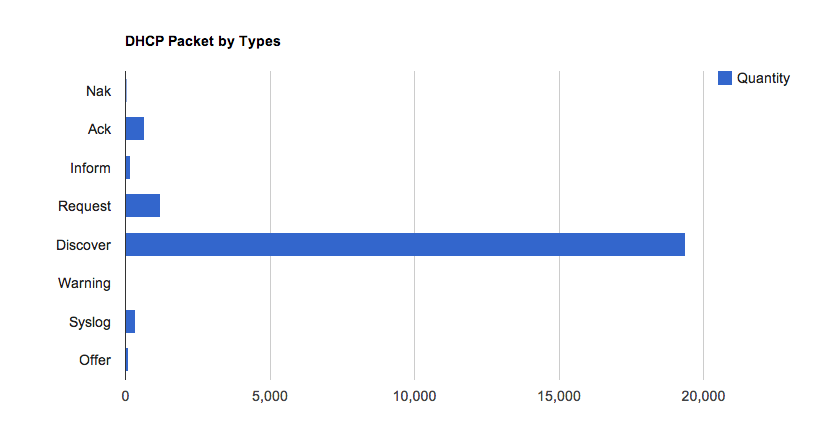
\includegraphics[width=1\textwidth]{Pictures/chapter5/dhcpCrash.png}
   \caption{DHCP Crash - 04/04/14}
\end{figure}

\section{RADIUS}
The analysis we made about the \texttt{RADIUS} are quite limited by the verbosity of the logs and by the fact that we do not have any direct access to the server. What we have chosen to monitor here are some general indicators.

\subsection{Authentication Success Rate}
The first thing we can observe about the \texttt{RADIUS} is the proportion of users being able to authenticate. If this rate drastically drops, that could indicate issues about the \texttt{RADIUS} server. This indicator alone does not bring much information but could be compared with the average authentication success rate to detect some important divergences.

\paragraph*{Overall Success Rate} The purpose of this graph is to get an idea of the average authentication success rate. Concretely, it counts the logs showing the messages \textit{login success} or \textit{fail}. Here again, we do not keep data about specific users. All the data are aggregated to compute the desired ratio. Each of these logs contains sensible information about the user and the time at which he established a connection with an AP. By crossing this information with the access point, we may follow his position throughout the day. We chose to limit this possibility by not linking those information together in the database. Even if this limitation could be easily broken, it's more an ethical consideration than a security issue.

\begin{figure}[H]
	\centering
   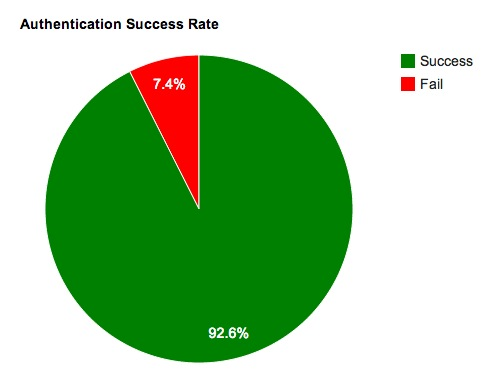
\includegraphics[width=0.5\textwidth]{Pictures/chapter5/radiusRate.jpg}
   \caption{Example of \texttt{RADIUS} Success Rate}
\end{figure} 

\paragraph*{Sources} The sources of those data are the \texttt{RADIUS} log files. These files contains an entry for each authentication attempt. Here is an example of the success and fail messages we find in the \texttt{RADIUS} log files.\\

\begin{lstlisting}[frame=single,breaklines=true,caption={\texttt{RADIUS} logs}]
2013-10-21T17:27:48+02:00 radius1.sri.ucl.ac.be radiusd[17913]: [ID 702911 local4.notice] Login incorrect: [XXXX] (from client WiSMPythagore-A port 29 cli XX-XX-XX-XX-XX-XX)
2013-10-21T17:27:50+02:00 radius1.sri.ucl.ac.be radiusd[17913]: [ID 702911 local4.notice] Login incorrect: [none] (from client WiSMPythagore-A port 29 cli XX-XX-XX-XX-XX-XX)
2013-10-21T17:27:55+02:00 radius1.sri.ucl.ac.be radiusd[1523]: [ID 702911 local3.notice] Login OK: [XXXX] (from client WiSMStevin-B port 29 cli XX-XX-XX-XX-XX-XX)
2013-10-21T17:27:55+02:00 radius1.sri.ucl.ac.be radiusd[1523]: [ID 702911 local3.notice] Login OK: [XXXX] (from client localhost port 0)
2013-10-21T17:27:59+02:00 radius1.sri.ucl.ac.be radiusd[1523]: [ID 702911 local3.notice] Login OK: [XXXX] (from client WiSMStevin-B port 29 cli XX-XX-XX-XX-XX-XX)
\end{lstlisting}

\section{Summary}
This chapter detailed the main results developed by our application from the data gathered with the \texttt{SNMP} protocol and the several log files. The main interest of gathering these data comes from the fact that they are linked together. Notice that all the data are already available on the controller but by trying to correlate some of them, we wanted to give another view of the network and shed light on some misunderstood issues. 

 
% Chapter Template

\chapter{Analysis and Results} % Main chapter title

\label{Chapter6} % Change X to a consecutive number; for referencing this chapter elsewhere, use \ref{ChapterX}

\lhead{Chapter 6. \emph{Analysis and Results}} % Change X to a consecutive number; this is for the header on each page - perhaps a shortened title

\section{Analysis}
The final purpose of our system is to provide analysis about the main issues present on the infrastructure. The way we process here is quite simple:

\begin{enumerate}
\item Putting together the related information
\item Spotting the anomalies
\item Trying to understand the causes
\end{enumerate}
Like in any system, we had to define domains on which the monitoring tool will be able to work. One of the first steps of this thesis was to determine what were or could be the main issues on the UCL's network. It's here that we will use those results. Each of these problems will be a domain in which we will define what are the relevant data, how they can help us and how to react after having analysed them. The purpose of this chapter is to present you these domains and the methodology used inside them. Each of them have their particular needs and their related techniques of analysis.

\section{Wifi}
\subsection{Users}
This section of the application offers some aggregated statistics about the users of the \emph{wifi network}. The main goal is to get some analysis of the actual utilization of the wireless infrastructure. It's more a set of indicators to help the administrators to get a global view of his network. 
\subsubsection*{Wifi Protocol}
This graph display the repartition of the users among the available \texttt{802.11} standards (i.e. 802.11a, b, g, n). The reason for this analysis comes from an earlier policy enforced on the UCL network that forbids the use of the \texttt{802.11b} protocol. Users connecting with such low bandwidth standard force the \emph{access point} to transmitting longer and can in consequence prevent the others to achieve higher receiving speed. Our analyse was created to help the administrators in future considerations in the same domain. By profiling the habits of the users, we can define the impact of such decision. As the quality of the service is one of the main concern, deactivating the utilization of a standard used by most of the devices could have heavy consequences.
The statistics are based by default on the connections of the last three months. It's to ensure that devices no longer using the network doesn't affect the result and keep the analyse as up to date as possible.
\paragraph*{Source:} The data used come from \texttt{SNMP}. At each cycle gathering the information of the \emph{devices} associated with the \emph{access points}, we get the information thanks to the value available on the controller. All the descriptions of the OIB come from the Cisco OID Browser \footnote{http://tools.cisco.com/Support/SNMP/do/BrowseOID.do}.

\begin{tabular}{|r l|}
\hline
\textbf{Object} & \texttt{bsnMobileStationProtocol} \\
\textbf{Description} & \parbox{11cm}{The 802.11 protocol type of the client. The protocol is mobile when this client detail is seen on the anchor i.e it's mobility status is anchor.} \\
\textbf{OID} & 1.3.6.1.4.1.14179.2.1.4.1.25 \\
\textbf{MIB} & AIRESPACE-WIRELESS-MIB \\
\hline
\end{tabular}

\subsubsection*{SSID Utilization}
Here, we count the number of users by \texttt{SSID}. As before, the goal is to provide a profile of the users to the administrators. Such measures can help to adapt the policies related to each \texttt{VLAN} and defining the load of each of them. It could help to diagnostic a useless \texttt{VLAN} or in the opposite, allow to detect an overloaded one that could be caused by an improper use of the network. The supposed utilization and the actual one can be really different and such indicators can help to adapt the configurations.
\paragraph*{Source:} As before, we mainly aggregate the data available on the controller.

\begin{tabular}{|r l|}
\hline
\textbf{Object} & \texttt{bsnMobileStationSsid} \\
\textbf{Description} & \parbox{11cm}{The SSID Advertised by Mobile Station.} \\
\textbf{OID} & 1.3.6.1.4.1.14179.2.1.4.1.7 \\
\textbf{MIB} & AIRESPACE-WIRELESS-MIB \\
\hline
\end{tabular}

\subsection{Access Point}
This section group several analysis related to the \emph{access points}. In a network with several hundreds of \emph{access point}, it can be difficult to diagnostic and monitor each one of them. By centralising and aggregating the data, we allow the network managers to save time by automatising lot of computation. In this part of the application, we have access to the monitoring of each access point currently associated with the controller.
\subsubsection{Population}

\subsubsection*{Load}
A fundamental piece of information related to an \emph{access point} is the load. To achieve that we monitor each spot continuously and record its state several times per hour. By analysing these data, we are able to plot graph representing the load throughout the days. To achieve that, we need two information: the \textit{quantity} of data transiting in the link and the \textit{maximum speed} of the link. Concretely, each \texttt{AP} own two bytes counters that are incremented each time a byte is received or sent. The other information required is the link speed connecting the spot. This information alone can be useful to diagnostic bandwidth issues. In a big network, it can be difficult to keep track of which links were updated and which ones were not. By collecting these data, we found that some \emph{access point} were still connected to \texttt{10 Mbits} links. In this case, the main cause was that the concerned devices were not managed by the same service and in consequence were not updated with the others. % ????
This is the proof that even such simple data can help to diagnostic some inconsistency in the network.
\paragraph*{Source:} Here again, we use the data available on the controller. The first data collected are the bytes counter of each \emph{access points}.

\begin{tabular}{|r l|}
\hline
\textbf{Object} & \texttt{cLApEthernetIfRxTotalBytes} \\
\textbf{Description} & \parbox{11cm}{This object represents total number of bytes in the error-free packets received on the interface.} \\
\textbf{OID} & 1.3.6.1.4.1.9.9.513.1.2.2.1.13 \\
\textbf{MIB} & CISCO-LWAPP-AP-MIB \\
\hline
\end{tabular}

\begin{tabular}{|r l|}
\hline
\textbf{Object} & \texttt{cLApEthernetIfTxTotalBytes} \\
\textbf{Description} & \parbox{11cm}{This object represents total number of bytes in the error-free packets transmitted on the interface.} \\
\textbf{OID} & 1.3.6.1.4.1.9.9.513.1.2.2.1.14 \\
\textbf{MIB} & CISCO-LWAPP-AP-MIB \\
\hline
\end{tabular}

The next step is to obtain the speed of each link connected to an \emph{access point}. This time again we use the \texttt{SNMP} protocol to get the information from the controller.

\begin{tabular}{|r l|}
\hline
\textbf{Object} & \texttt{cLApEthernetIfLinkSpeed} \\
\textbf{Description} & \parbox{11cm}{Speed of the interface in units of 1,000,000 bits per second.} \\
\textbf{OID} & 1.3.6.1.4.1.9.9.513.1.2.2.1.11 \\
\textbf{MIB} & CISCO-LWAPP-AP-MIB \\
\hline
\end{tabular}

\subsubsection*{Interfaces}
Each \emph{access point} has two wifi interfaces. The first one emits at \texttt{5Ghz} and the second on \texttt{2,4Ghz}. For each interface, the controller provides a lot of information completing the previous ones. The first that we gather is the \textit{number of users} currently associated to the interface. We compare these data with the quantity of users with a poor \texttt{Signal-Noise Ratio} (SNR). This analysis allows to diagnostic the efficiency of the access point. Even if it can be considered normal to have a couple of users in this category, if the proportion is constantly high, it can be an indicator that a supplementary \emph{access point} may be helpful or that the location of the AP is problematic. The problem have to be put in perspective with the statistics of the number of users and the RF environment (i.e \emph{Rogue Access Point} or physical walls) which is outside the scope of this system. 
Finally, we complete this analyse with a monitoring of the \emph{channel utilization}. A high utilization of the channel results in poor connection quality for the user and could indicates a poor RF condition.

\paragraph*{Source:} The controller keeps entries for each interface of each access point. We gather and cross all these data to generate some logs about each \emph{access point} and all the related \emph{interfaces}.

\begin{tabular}{|r l|}
\hline
\textbf{Object} & \texttt{bsnAPIfLoadNumOfClients} \\
\textbf{Description} & \parbox{11cm}{This is the number of clients attached to this Airespace AP at the last measurement interval.} \\
\textbf{OID} & 1.3.6.1.4.1.14179.2.2.13.1.4 \\
\textbf{MIB} & AIRESPACE-WIRELESS-MIB \\
\hline
\end{tabular}

\begin{tabular}{|r l|}
\hline
\textbf{Object} & \texttt{bsnAPIfPoorSNRClients} \\
\textbf{Description} & \parbox{11cm}{This is the number of clients with poor SNR attached to this Airespace AP at the last measurement interval.} \\
\textbf{OID} & 1.3.6.1.4.1.14179.2.2.13.1.24 \\
\textbf{MIB} & AIRESPACE-WIRELESS-MIB \\
\hline
\end{tabular}

\begin{tabular}{|r l|}
\hline
\textbf{Object} & \texttt{bsnAPIfLoadChannelUtilization} \\
\textbf{Description} & \parbox{11cm}{Channel Utilization.} \\
\textbf{OID} & 1.3.6.1.4.1.14179.2.2.13.1.3 \\
\textbf{MIB} & AIRESPACE-WIRELESS-MIB \\
\hline
\end{tabular}



\subsection{Rogue Access Points}

\subsection{Simulation of a user}
We use our \texttt{OpenWrt} routers as probes that simulate the behavior of a lamba user that connects to the university network. In order to do that, we have implemented a \texttt{C} program using \texttt{wpa\_supplicant} and its control interface. This program, launched by the router at boot, tries to establish a connection with each one of the five \texttt{VLANs} of the UCL (i.e. \texttt{student.UCLouvain}, \texttt{UCLouvain}, \texttt{visiteurs.UCLouvain}, \texttt{UCLouvain-prive} and \texttt{eduroam}). During that connection process we compute the time taken by \texttt{wpa\_supplicant} to get a connection and the time taken by \texttt{udhcpc} to get an IP address. Thanks to those information we can approximate the overall quality perceived by the normal users when they want to get an access to the Internet inside the UCL. Beside that, our program also checks if a selection of the most used services by a user are reachable with each of the \texttt{VLANs}. We have decided to check the reachability of the following services:
\begin{itemize}
	\item[-] \texttt{www.google.be}
	\item[-] \texttt{www.smtp.gmail.com}
	\item[-] \texttt{www.github.com}
	\item[-] \texttt{www.uclouvain.be}
	\item[-] \texttt{www.icampus.uclouvain.be}
\end{itemize}

We add these additional information to the log file our program creates and sends to our server for parsing and analysis.

\subsubsection*{Choice of the Access Point}
The first thing our program does when it starts its connection loop is to perform a scan of the networks available where the probe is placed and to write the results inside the log file. Among the results and for each network we have decided to keep the network \texttt{BSSID}, the \texttt{Signal Strength} of the network and its \texttt{SSID}. Those data are interesting for our analysis. Indeed, when the router tries to get a connection, it first tries to associate with an Access Point. But there could be several APs in the area and he might be rejected from one or several of them. If its association request is rejected by one AP, \texttt{wpa\_supplicant} will try to associate with another one, and so on until the request is accepted. Our program gathers all the \texttt{BSSID} of the APs it had an association request with. 
Comparing the scan results for each AP and the APs tried and the one it has a connection with is quite interesting. Indeed, after having performed several tests, we have observed that the device does not always connect to the best AP (i.e. the one with the best signal strength).

One explaination for that is that in its choosing process, %https://chromium-review.googlesource.com/#/c/183720/

\section{Controller}
The controller logs are divided in several categories. Each of them defined a list of log related to that category. The main idea here is to analyse the activity of each domain of logs and trying to spot irregularities. We make the hypothesis that when something went wrong, the related category will emit a larger number of logs. By monitoring that activity, we will be able to identified in which part of the infrastructure the issue happened.

\subsection{Components Activity}


\section{DHCP}
These analyses aim to detect \emph{DHCP} related issues. The allocation  of IP addresses is a fundamentals component in our network. Being able to detect when problems appears and advertise them could help to make a quicker and more efficient response.

\subsection{Leases}
The main problem with a DHCP is the allocation of ranges of addresses. It's always difficult to determine the quantity of required IP by VLAN. Moreover, when such problems arise, it can be hard to be aware of them. Most of the time, users don't report the problem and when they do, their descriptions state only that they can't connect which is not very useful. Being able to automatically detect a lack of IP addresses can be very time saving for any administrators. Even is such information are available in the \emph{DHCP} logs and that the servers could send warnings, centralising these information aside data related to all the other components of the infrastructure can lead to more powerful analysis. 

\subsection{Crash}


\section{Radius}


\subsection{Authentication Success Rate}




 
% Chapter Template

\chapter{Conclusion and Future Talks} % Main chapter title

\label{Chapter 7} % Change X to a consecutive number; for referencing this chapter elsewhere, use \ref{ChapterX}

\lhead{Chapter 7. \emph{Conclusion and Future Talks}} % Change X to a consecutive number; this is for the header on each page - perhaps a shortened title

%----------------------------------------------------------------------------------------
%	SECTION 1
%----------------------------------------------------------------------------------------
\section{Beta Version}
As we conclude this project, we wanted to remind you that this is only a \emph{beta} version and a lot of improvements can be done. About one year ago, we have started from scratch with few knowledge of the UCL infrastructure and how most of the used protocols work. Today, we have an application that is able to analyse and has a basic understanding of the data it deals with. Like most of new project, we used a lot of time in the design of the architecture. We think that it is the most important when we want to ensure a possible future to our system. We hope that our thesis will be continued by future students and we wonder that it become a complete monitoring tool. Modularity and maintainability were our two main concerns.

\section{Portability}


\section{Ethical Considerations}
% introduite dans le ch5->logparser->radius
Several time we needed to limit the possibility of the application. The goal of the system is to offer a global view to the network administrators and giving them the most possible information. So, we have started to implement basic features to get the simplest pieces of data. Once that was done, we have listed the possible information that could be generated by crossing the data and implement the ad hoc methods. Quickly, it appears that the capabilities of the application could become sensitive. We have taken care of generating a modular infrastructure that make easy the creation of new analysis but some of them can be seen as unethical. For example, the \emph{radius logs} make possible to trace an user through the day and represent his position on a map. Such features could seem useful to detect and to diagnostic precisely a problem but we have chosen to not implement them. The question was "where the limit is?" and to answer it we simply used the requirements of the network administrators. We have translated them to a \emph{goal model} and for each goal we tried to find the proper answer. It appears that most of them was solvable by aggregating the data. By proceeding in that way, we completely un-personalized the information. 
Nevertheless, we can't bride completely the system and ensure a complete ethical utilization of it. We think it's really important to keep in mind that, even if the purpose is to offer a better service, the privacy is an important concern when we choose to extends the project.

%----------------------------------------------------------------------------------------
%	THESIS CONTENT - APPENDICES
%----------------------------------------------------------------------------------------

\appendix % Cue to tell LaTeX that the following 'chapters' are Appendices

% Include the appendices of the thesis as separate files from the Appendices folder
% Uncomment the lines as you write the Appendices

% Appendix Template


\chapter{Source Code} % Main appendix title
\label{AppendixA} % Change X to a consecutive letter; for referencing this appendix elsewhere, use \ref{AppendixX}
\lhead{Appendix A. \emph{Source Code}} % Change X to a consecutive letter; this is for the header on each page - perhaps a shortened title

The source code of our monitoring application is available on Github at the following address: \texttt{https://github.com/cwayembergh/netwobserver/}.
Here is the list and descriptions of the contents of this repository.

\begin{itemize}
\item[-] \texttt{analyse/}: Module that performs analysis and aggregations on the data.
\item[-] \texttt{analyse/observation/monitoring.py}: Methods detecting the anomalies.
\item[-] \texttt{analyse/computation/aggregation.py}: Methods performing the aggregations and computations on the data.
\item[-] \texttt{gatherer/}: Module that is responsible to gather the data.
\item[-] \texttt{gatherer/log/}: Module that performs the parsing of the log files.
\item[-] \texttt{gatherer/snmp/}: Abstractions for the SNMP requests.
\item[-] \texttt{gatherer/probe/}: Module that manage the connections with the probes.
\item[-] \texttt{netwObserver/settings.py}: Settings of the application. Contains the user preferences.
\end{itemize}




\backmatter
%----------------------------------------------------------------------------------------
%	BIBLIOGRAPHY
%----------------------------------------------------------------------------------------
\label{Bibliography}
\lhead{\emph{Bibliography}}
\bibliography{Bibliographie/Bibliography.bib}
\bibliographystyle{unsrtnat}


\end{document}